\documentclass[../thesis/thesis.tex]{subfiles}
\begin{document}

\chapter{Design}
\label{chap:design}

In this chapter, we explain the methodology used to fill the research gap identified in Chapter~\ref{chap:litreview}, thereby producing a system that identifies high-potential startup companies that are likely to receive additional funding or a exit in a given forecast window. Figure~\ref{fig:design:system_architecture} depicts the overall system architecture, which is described in the following chapter. We evaluate the performance of this system in the next chapter.

\begin{figure}[!htb]
    \centering
    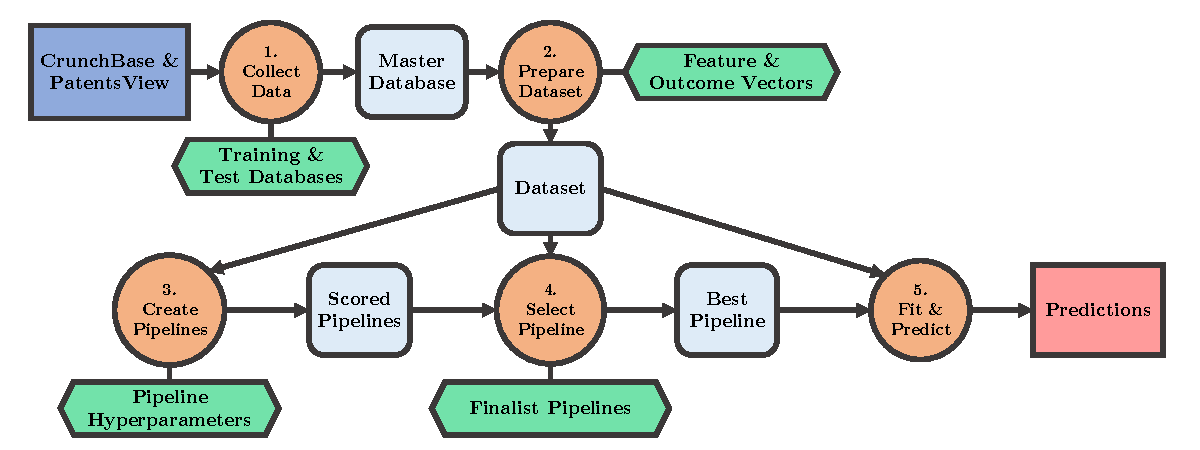
\includegraphics[width=\textwidth]{../figures/design/flowchart_overview}
    \caption[System architecture flowchart]{An overview of the system architecture proposed by this project, structured in four stages: data collection, pipeline creation, pipeline selection and prediction. Legend: dark blue square = input, yellow circle = process, light blue rounded square = intermediate, red square = output, green hexagon: iterative process / search space.}
    \label{fig:design:system_architecture}
\end{figure}

\begin{enumerate}

\item Dataset Preparation. We developed a conceptual framework of startup investment from the literature to guide our feature and data source selection. We selected CrunchBase, a startup database, as our primary data source, which we supplemented with patent filing records from PatentsView. We collected two database dumps from CrunchBase in September 2016 and April 2017, for training and testing respectively. The database dumps were in the format of CSV files which we imported into a relational database (SQLite) and performed aggregation queries to create features suitable for classification. We then performed screening based on each company's developmental stage and age to ensure only relevant companies were included in the dataset. Finally, we explored the dataset and identified issues of sparsity, long-tailed distributions, imbalanced feature ranges, and non-orthogonality.

\item Pipeline Creation. We developed a processing pipeline framework that seeks to address the dataset issues identified during data collection. Our pipeline is based on the popular Python machine learning library Scikit-learn \cite{pedregosa2011}. Pre-processing steps include imputation, transformation, scaling and feature extraction. Each pre-processing step has hyper-parameters that can be tuned (e.g. imputation strategy, number of components to extract) that affect the pipeline's classification performance. We also tested a number of common classification algorithms and their hyper-parameters, selected from our literature review in Chapter~\ref{chap:litreview}. We performed a search across the pipeline's hyper-parameters to generate candidate pipelines. The hyper-parameters that we found to have the most significant effect on the final performance of the pipelines were related to the classification algorithms.

\item Pipeline Selection. Our system evaluates and ranks the candidate pipelines and tests the best pipelines (finalist pipelines) over pseudo-historical datasets. This process ensures we select pipelines that are robust with respect to time. We prepared the dataset slices using a technique that filters records by their timestamps, effectively recreating historical datasets. We use Area under \gls{pr} Curve as our evaluation metric. We aggregate the results for each finalist pipeline across these dataset slices and rank the finalist pipelines on their overall performance, so we can select the best pipeline for further evaluation. We don't observe significant variance in the pipelines on aggregate against the dataset slices, but there is variance within the individual pipelines. Our results suggest that it is optimal to evaluate the top 3-5 candidate pipelines in this manner.

\item Model Fit and Prediction. Finally, our system applies the best pipeline to a training dataset to produce a fitted model. The model is then applied to a feature vector from a held-out test database, which generates a set of predictions which could, in practice, then be used by \gls{vc} firms. We evaluate the accuracy of the models produced by our system with respect to a number of variables in the next chapter.

\end{enumerate}

\section{Dataset Preparation}

In the previous chapter, we reviewed the literature concerning feature selection and data sources for entrepreneurship and \gls{vc} investment. We identified that a wide range of features have been implicated as significant to startup performance, but concluded that the field is lacking a unified conceptual framework. We evaluated that the most promising primary data sources for this project are CrunchBase and AngelList, for their size, comprehensiveness and ease of access. We suggested PatentsView (the online database of the US Patent Office) could be a useful secondary data source for structural capital features.

In this section, we first discuss how we developed a conceptual framework that guided our feature and data source selection. Next, we describe the process of generating our primary datasets, which involves collecting data from CrunchBase and PatentsView, converting the relational databases into a format suitable for machine learning, and performing screening to ensure we only included relevant companies. This process is depicted in Figure~\ref{fig:design:data_collection}. Finally, we describe the results of our exploratory analysis and identify dataset issues to be addressed in later steps.

\begin{figure}[!htb]
    \centering
    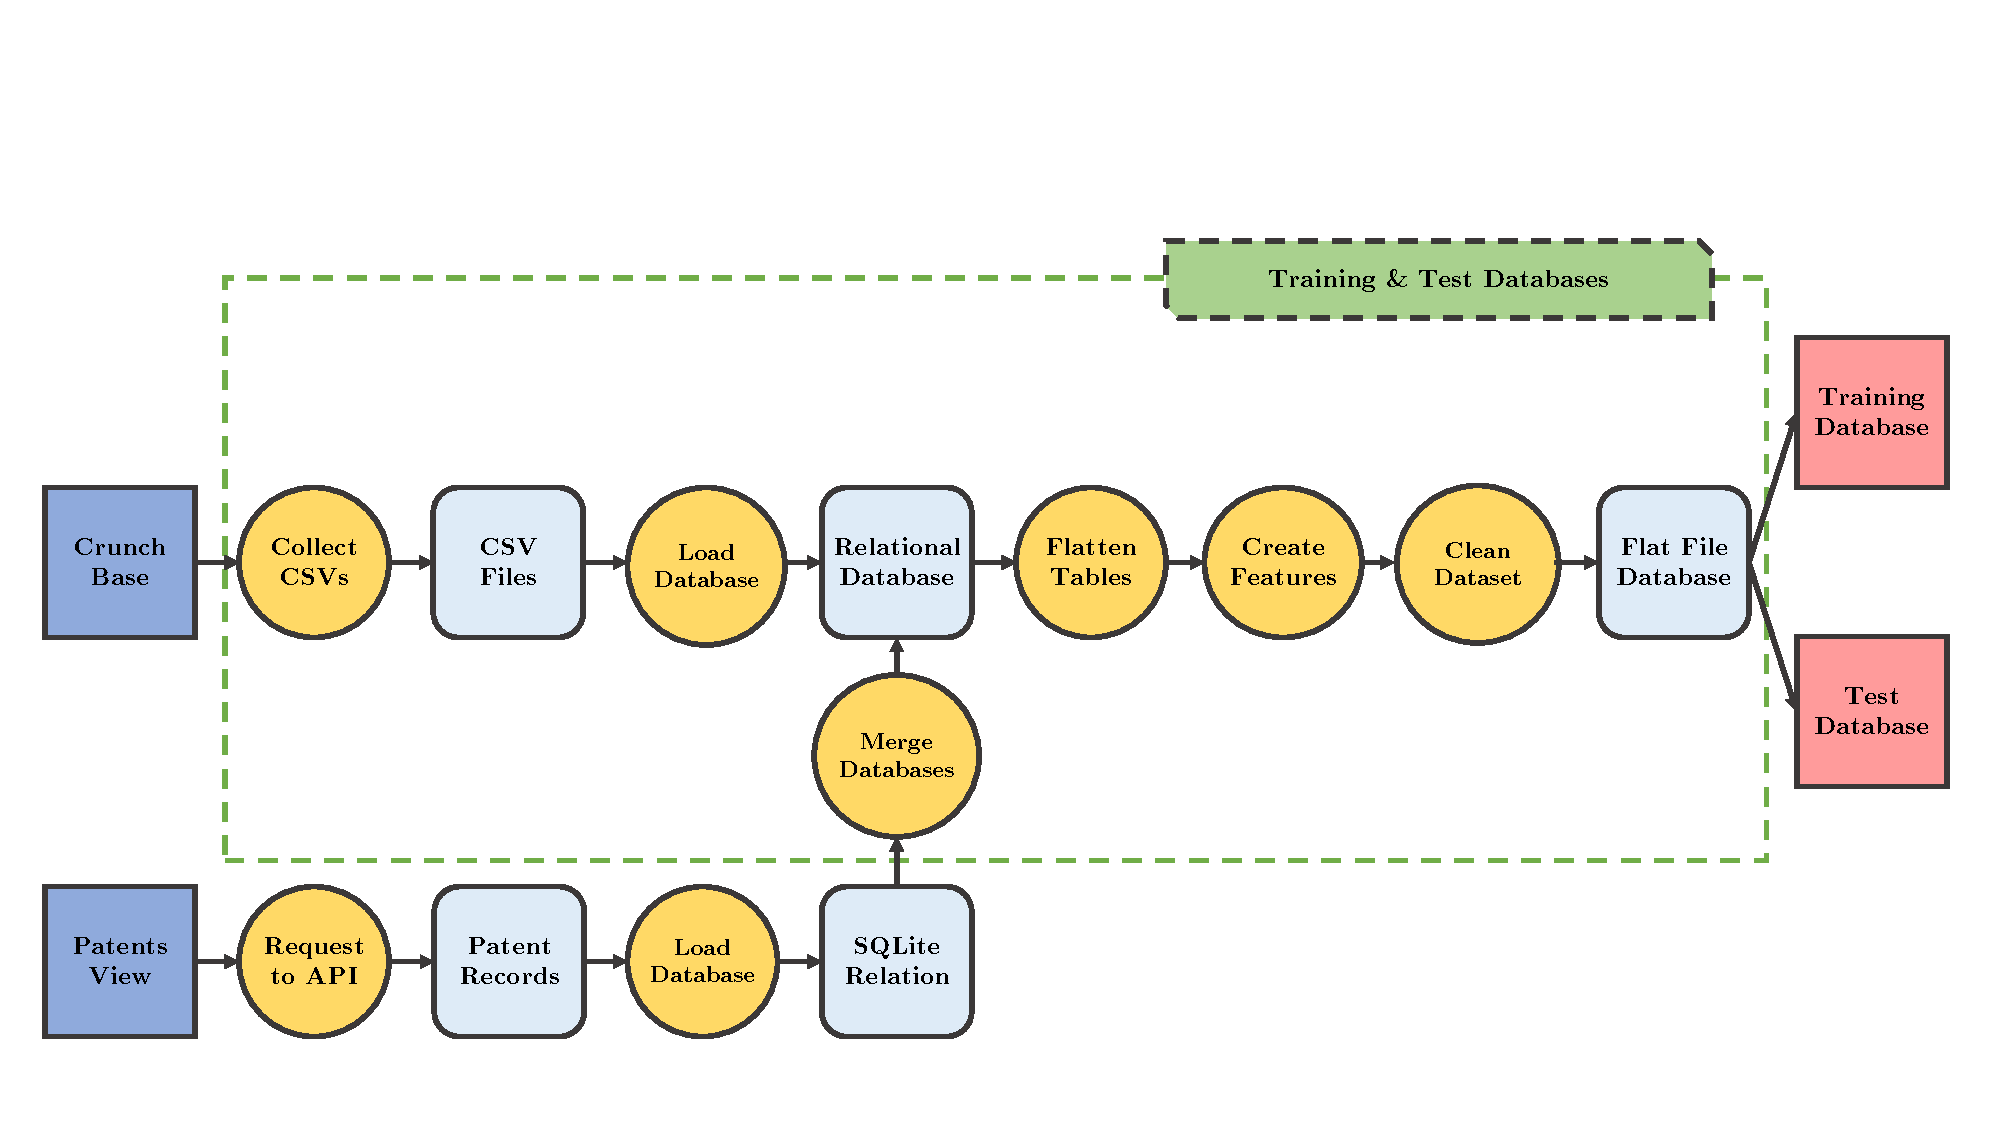
\includegraphics[width=\textwidth]{../figures/design/flowchart_data_collection}
    \caption[Data collection flowchart]{Data collection overview. Legend: dark blue square = input, yellow circle = process, light blue rounded square = intermediate, red square = output, green hexagon: iterative process / search space.}
    \label{fig:design:data_collection}
\end{figure}

\subsection{Feature Selection}

We developed a conceptual framework that builds upon previous work to ensure that we include a comprehensive and relevant set of features in our investment screening system. This framework builds on previous work by Ahlers and colleagues (2015), designed to model performance on equity crowd-funding platforms \cite{ahlers2015}. We sought to generalise Ahlers' framework~\cite{ahlers2015} beyond equity crowd-funding. While the first factor of Ahlers' framework (venture quality) applies to startups generally, Ahlers defined their second factor (investment confidence) with respect to whether startups offer an equity share in their crowd-funding, and whether they provide financial projections. These features are specific to equity crowd-funding. We proposed an extension of Ahlers' framework that generalises and develops this second factor. We described investment confidence as a product of third party validation, historical performance and contextual cues. Our proposed framework is depicted in Figure~\ref{fig:design:features:framework_simple}.

\begin{figure}[!htb]
    \centering
    
\begin{forest}
    forked edges,
    for tree={
        grow=west,
        align=center,
        l sep = 2cm,
        fork sep = 1cm,
        child anchor=east,
        anchor=base east,
        tier/.pgfmath=level(),
        edge={<-, thick},
        every node={rectangle,draw=black}
    }
[Startup\\Investment,
    [Startup\\Potential,
        [Human Capital]
        [Social Capital]
        [Structural Capital]
    ]
    [Investment\\Confidence,
        [Third Party Validation]
        [Historical Performance]
        [Contextual Cues]
    ]
]
\end{forest}

    \caption[Conceptual framework for startup investment.]{Proposed conceptual framework for startup investment. We adapt the framework proposed by Ahlers et al.~\cite{ahlers2015}, originally based on work by Baum and Silverman~\cite{baum2004}. For an extended version of this framework, please refer to Figure~\ref{fig:appendix:features:framework_details}.}
    \label{fig:design:features:framework_simple}
\end{figure}

Feature selection is critical to the success of our proposed conceptual framework. In this section, we have built on the framework proposed by Ahlers et al. \cite{ahlers2015} in several ways. First, our framework generalises the ``Investment Confidence'' factor for startups seeking any type of investment (not just equity crowd-funding). Second, our framework has greater depth. Where Ahlers uses one or two features for each factor in their model (e.g. ``\% Non-executive board'' represents ``Social (alliance) capital''), we perform a review of many features employed in this area and perform a higher degree of classification. For example, in our proposed framework ``Social (alliance) capital'' is composed of ``Social media influence'', ``Events influence'' and ``Strategic alliances'', each of which will also be composed of several features (e.g. ``Twitter followers'', ``Average Tweets per day'').

%BLah blah CrunchBase & PatentsView

\subsection{Data Collection}

\subsubsection{CrunchBase}

We were granted an Academic License to collect data from CrunchBase. CrunchBase provides database access in a few formats that offer trade-offs in terms of accessibility and comprehensiveness: REST API, CSV Dumps, MS Excel Summary. We chose to use the CSV Dumps for this implementation of the system because they provided a good trade-off of ease of use and comprehensiveness of access. The Dumps provide a CSV file for each of CrunchBase's key endpoints (e.g. organizations, people, funding rounds) which can be loaded easily into relational databases (see Appendix~\ref{appendix:database_schema} for the database schema). We downloaded CSV Dumps from CrunchBase on 09 September 2016 and 04 April 2017 which became our training and testing datasets, respectively.

\subsubsection{PatentsView}

We used PatentsView to obtain the patent filing records of each company in our CrunchBase dataset, focusing on information relating to dates, citations, and patent types. We matched the data sources on standardised company names (removing common suffixes, punctuation etc.) and using normalised Levenshtein distances. Although approximate matching introduces error, the volume of companies in the database is too high to be matched manually and there are no other identifying records. We stored the PatentsView data in a relation which we merged into our master and test databases.

\subsection{Dataset Manipulation}

To prepare the dataset for machine learning, we first flattened the relational database into a single file using SQL aggregation queries. We aggregated each relevant relation in turn, grouping by Company ID and then combined each aggregated table using left outer joins. Following this process, we used Python to convert tuples (e.g. Round Type and Round Date) and lists (e.g. Round Types) into dummy variables.

We performed preliminary screening on the primary dataset (N = 425,934) to ensure it only included relevant companies. We were interested in removing traditional, non-startup businesses from the dataset (e.g. consulting firms, companies that will not take \gls{vc} funding etc.). To do this, we explored two factors for each company: developmental stage and age. By developmental stage, we primarily refer to external funding milestones. These stages are associated with shifts in a startup company's functions and objectives and we also expect them to correlate with company age. Our dataset as grouped by startup developmental stage is depicted in Figure~\ref{fig:design:lifecycle}.

\begin{figure}[!htb]
    \centering
    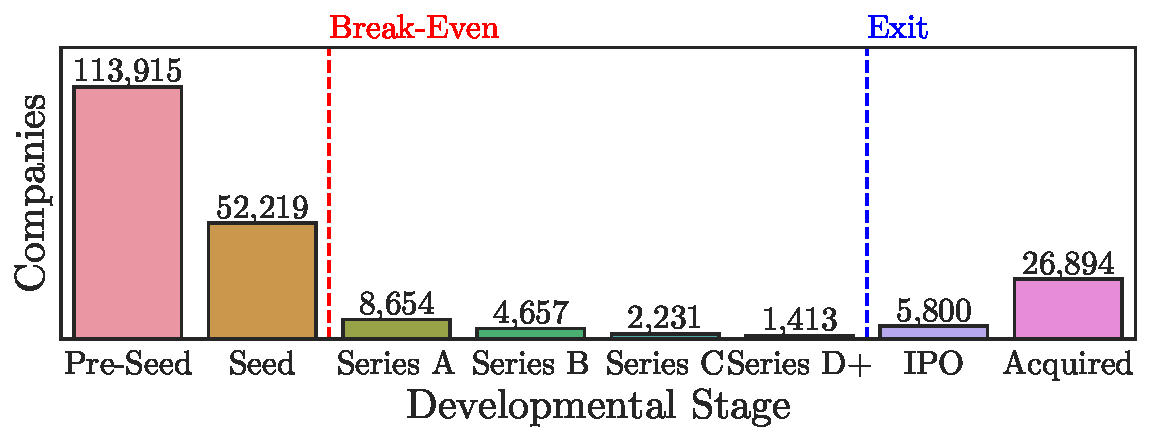
\includegraphics[width=\textwidth]{../figures/design/descriptives_counts_stage}
    \caption[Startup development life-cycle]{Companies grouped by stages of the startup development life-cycle.}
    \label{fig:design:lifecycle}
\end{figure}

After attempting to place the companies into development stages we are left with a large group of companies (the majority of the dataset) that have not raised funding and so can not be classified on that basis. We assume that companies that have not raised funding fall into two groups - those that intend to raise funding but have not had time to yet, and those that have chosen not to pursue funding and are unlikely to do so. We separated these groups by applying a cut-off equal to the 90th percentile of the age of companies in the Seed category, and excluded the older group from further analyses (N = 227,162,  53.3\%). As we are only interested in companies that could theoretically seek investment, we also excluded Closed, Acquired and IPO groups from further analyses (N = 35,973, 8.4\%).

Figure~\ref{fig:design:stages_ages} depicts the ages of companies in the master dataset, grouped by developmental stage. While there is significant variability in age for each developmental stage, there is a broad positive relationship between age and developmental stage. Most pre-Series A companies are under five years old, and the majority of Series D+ funded companies are under 10 years old and the 75th percentile is at 15 years old. On this basis, we excluded companies that are over the 75th percentile of the age of companies in the Series D+ category (N =9,756, 2.2\%). Overall, our preliminary screening steps reduced the dataset from 425,934 companies to 153,043 companies, a reduction of 64.1\%.

\begin{figure}[!htb]
    \centering
    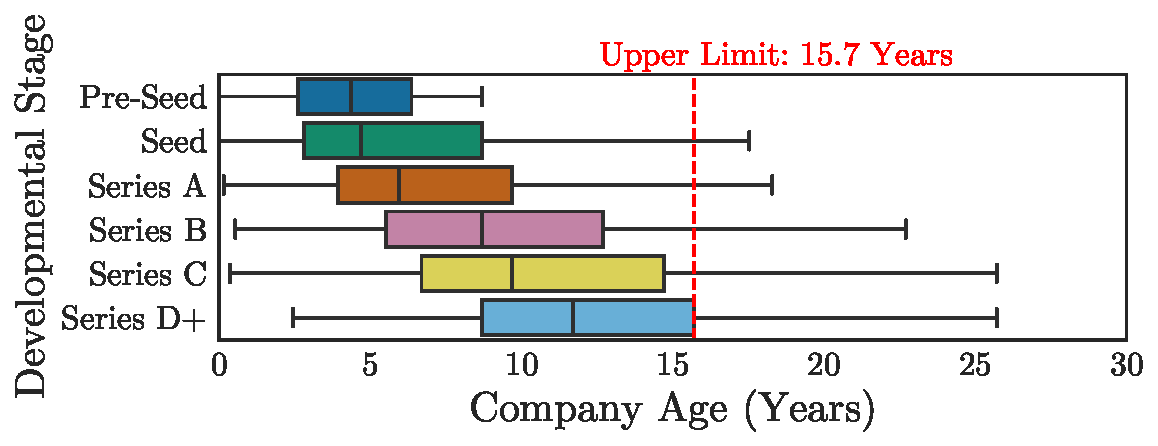
\includegraphics[width=\textwidth]{../figures/design/descriptives_ages_stage}
    \caption[Company ages by developmental stage]{Company ages in years grouped by developmental stage. The dashed red line represents the 75th percentile of the age of companies in the Series D+ category (15.7 years).}
    \label{fig:design:stages_ages}
\end{figure}

\subsection{Exploratory Analysis}

\subsubsection{Descriptive Statistics}

Table~\ref{tab:design:descriptive_statistics} presents the descriptive statistics for the dataset. The dataset is heavily skewed towards Pre-Seed companies (i.e. companies that were recently founded and have not raised any type of funding yet, 68.9\%). These companies have few available features in comparison to companies at later developmental stages. We will investigate the impact of this sparsity on our predictions in Chapter~\ref{chap:evaluation}. We are presented with a heterogeneous dataset: the interquartile ranges imply significant variability in all measures. We do not believe that this implies that the data has not been cleaned effectively, but rather, reflects that startup companies vary significantly in their traits.

\begin{table}[!htb]
    \centering
    \scalebox{0.9}{\begin{tabular}{lrrrrrrrrrrr}
\toprule
Stage &	Obs &
\multicolumn{2}{c}{\thead{Age\\(Years)}} &
\multicolumn{2}{c}{\thead{Funding Raised\\(USD, M)}}	&
\multicolumn{2}{c}{\thead{Funding\\Rounds (N)}}	&
\multicolumn{2}{c}{\thead{Patent\\Filings (N)}}	&
\multicolumn{2}{c}{\thead{Available\\Features (N)}}	\\
{}          & N         & 50th  & 75th  & 50th  & 75th  & 50th  & 75th  & 75th  & 90th  & 50th  & 75th \\ \midrule
Pre-Seed    & 113,915   & 4.36  & 6.36  & 0.00  & 0.00  & 0     & 0     & 0     & 0     & 25    & 133 \\
Seed        & 38,942    & 4.66  & 6.69  & 0.25  & 1.30  & 1     & 2     & 0     & 1     & 178   & 231 \\
Series A    & 6,615     & 5.69  & 8.70  & 4.40  & 9.41  & 2     & 3     & 0     & 2     & 239   & 302 \\
Series B    & 3,342     & 7.61  & 10.70 & 14.89 & 28.20 & 3     & 4     & 0     & 4     & 255   & 314 \\
Series C    & 1,610     & 8.70  & 11.70 & 35.29 & 62.00 & 3     & 5     & 1     & 9     & 305   & 321 \\
Series D+   & 998       & 9.70  & 12.70 & 74.39 & 130.8 & 5     & 7     & 4     & 19    & 319   & 330 \\
Included    & 165,422   & 4.69  & 6.69  & 0.00  & 4.00  & 1     & 2     & 0     & 1     & 90    & 160 \\
\bottomrule
\end{tabular}
}
    \caption[Descriptive statistics by developmental stage]{Descriptive statistics grouped by developmental stage.}
    \label{tab:design:descriptive_statistics}
\end{table}

CrunchBase's approach to industry classification is simplistic compared to other classification schemes (e.g., USSIC, NAICS, VentureSource) which generally have an industry hierarchy with tiers for broad industry sectors and sub-sectors providing further granularity. As a result, CrunchBase class labels include over represented and vague classes (e.g., ``Software'', ``Internet Services'') which could describe the majority of companies included in the database. In fact, ``Software'' and ``Internet Services'' account for 16.4\% and 13.4\% of all companies in the dataset respectively (see Figure~\ref{fig:design:industry_counts}). Despite these vague class labels, it is clear the dataset skews towards high technology startups, as opposed to biomedical, agricultural, or other technologies (which do not make the Top 10).

\begin{figure}[!htb]
    \centering
    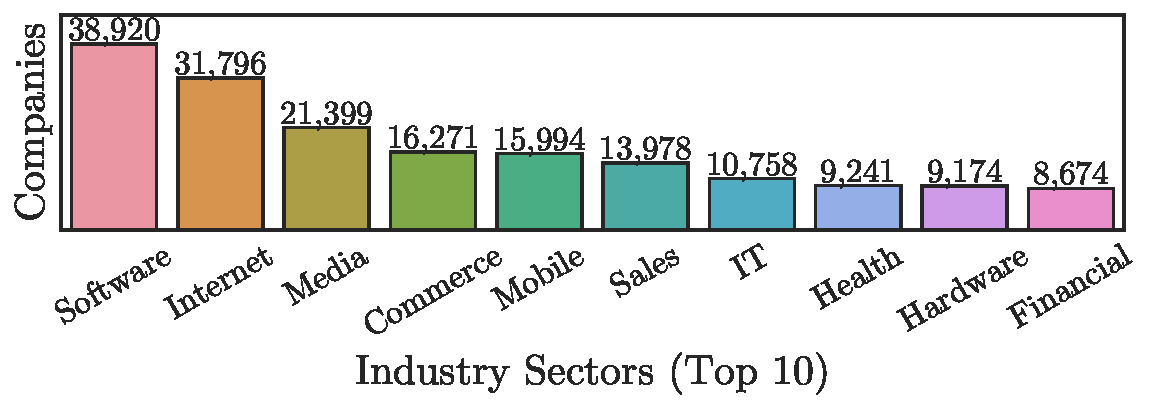
\includegraphics[width=\textwidth]{../figures/design/descriptives_counts_industry}
    \caption[Company counts by industry sector]{Companies grouped by industry sector. The 10 most common sectors are displayed. Source: Master dataset (c. September 2016).}
    \label{fig:design:industry_counts}
\end{figure}

\subsubsection{Sparsity} %Confusing figures

First, we explored missing data in the dataset. We expected the dataset to be highly sparse because it primarily came from CrunchBase, a crowd-sourced database. As profiles are entered into CrunchBase piece-meal, it is not clear at face-value whether data (e.g. records of funding rounds) is missing or didn't occur. Figure~\ref{fig:design:sparsity} displays the distribution of missing data in the dataset, with respect to each feature and each observation. The multi-modal peaks of both distributions suggest that missing data across certain groups of features may be correlated with each other (e.g. all features derived from funding rounds).

\begin{figure}[!htb]
    \centering
    \begin{subfigure}{\textwidth}
        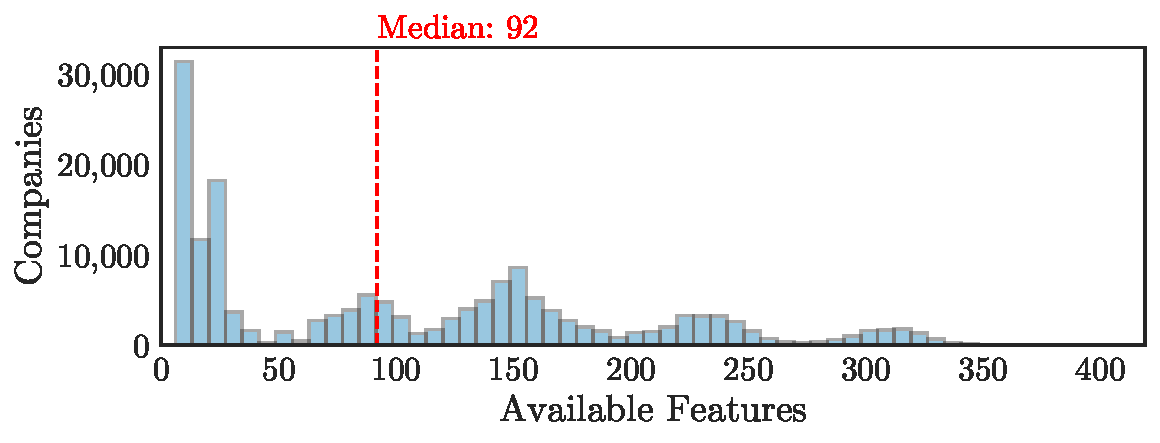
\includegraphics[width=\textwidth]{../figures/design/sparsity_features}
        \caption[Sparsity by company]{Distribution of missing data by company}
        \label{fig:design:sparsity:features}
    \end{subfigure}
    \begin{subfigure}{\textwidth}
        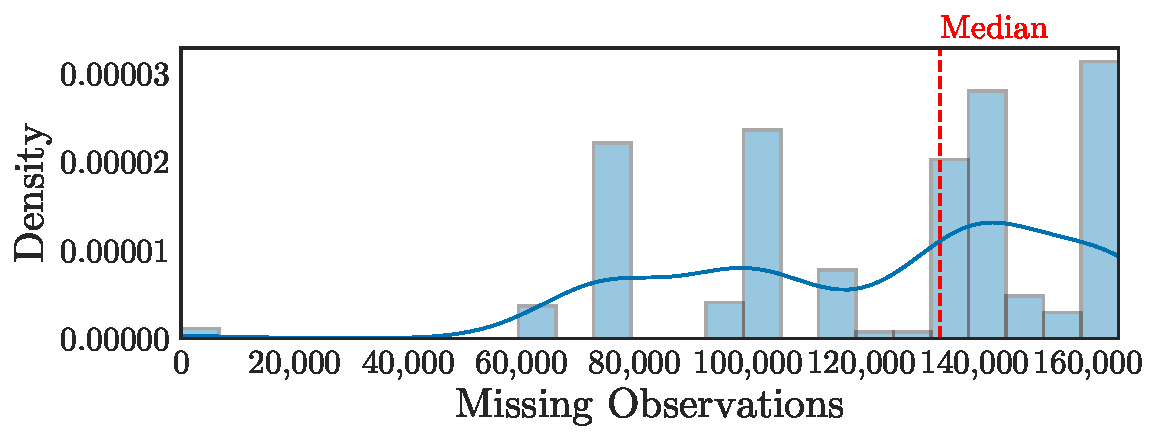
\includegraphics[width=\textwidth]{../figures/design/sparsity_observations}
        \caption[Sparsity by feature]{Distribution of missing data by feature}
        \label{fig:design:sparsity:observations}
    \end{subfigure}
    \caption[Distribution of missing data]{Distribution of missing data in master dataset (c. September 2016).}
    \label{fig:design:sparsity}
\end{figure}

\subsubsection{Normality} %Needs more explanation

Next, we explored the distributions of features. Figure~\ref{fig:design:normality} shows the skewness and kurtosis of the features in our dataset. A feature is considered horizontally symmetrical if it has a skewness of 0 and considered highly skewed if its absolute skewness is above 1 \cite{bulmer1979}. The vast majority of our features are more skewed than this cut-off. Kurtosis is a measure of the distribution of variance in a feature. We use Fisher's measure of kurtosis, which has a normal value of 0. Our dataset has consistently higher kurtosis than normal which suggests that we have many extreme values in our dataset. These results in concert suggest that our dataset has many features that are positively skewed with long-tail distributions. This is intuitively what we might expect for features like ``amount of funding raised''.

\begin{figure}[!htb]
    \centering
    \begin{subfigure}{\textwidth}
        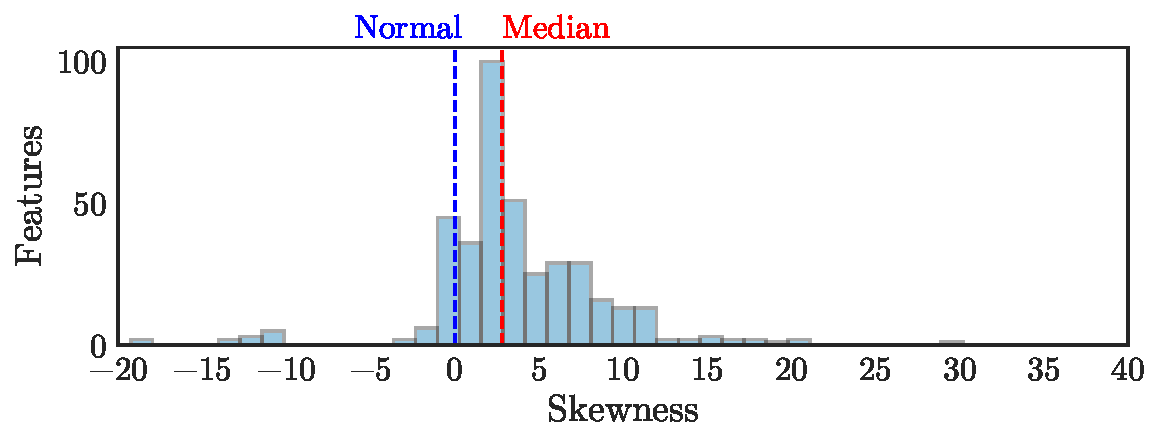
\includegraphics[width=\textwidth]{../figures/design/distribution_skew}
        \caption[Distribution of skewness by feature]{Skewness.}
        \label{fig:design:normality:skew}
    \end{subfigure}
    \begin{subfigure}{\textwidth}
        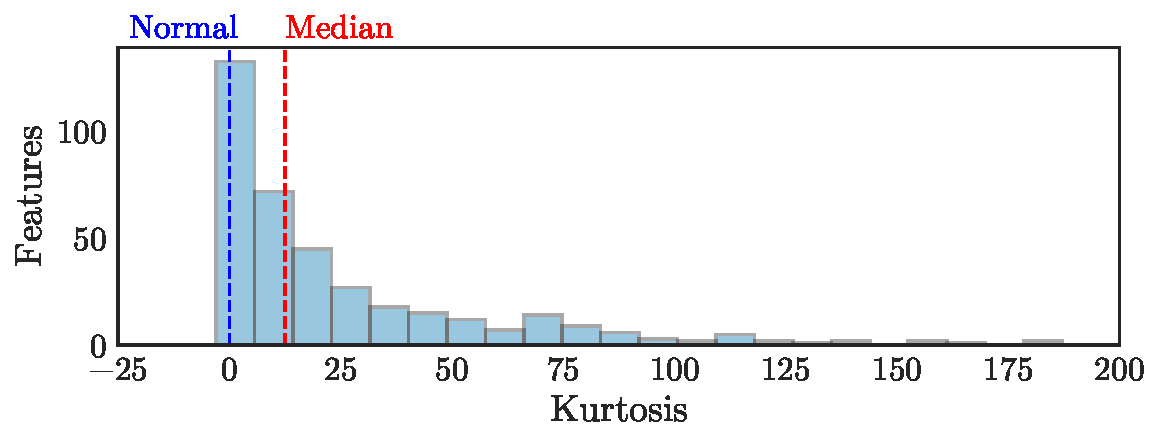
\includegraphics[width=\textwidth]{../figures/design/distribution_kurtosis}
        \caption[Distribution of kurtosis by feature]{Kurtosis.}
        \label{fig:design:normality:kurtosis}
    \end{subfigure}
    \caption[Distribution of skewness and kurtosis]{Distribution of features in master dataset (c. September 2016).}
    \label{fig:design:normality}
\end{figure}

\subsubsection{Scale}

Next, we explored the scaling and range of each of our features. Figure~\ref{fig:design:scaling} shows the \gls{iqr} of each feature (transformed by log1p for ease of viewing). The distribution is extremely skewed, which shows that our features have a wide range of magnitudes. This may be an issue for our machine learning estimators and feature extractors, so we address this by applying a scaler in our pipeline.

\begin{figure}[!htb]
    \centering
    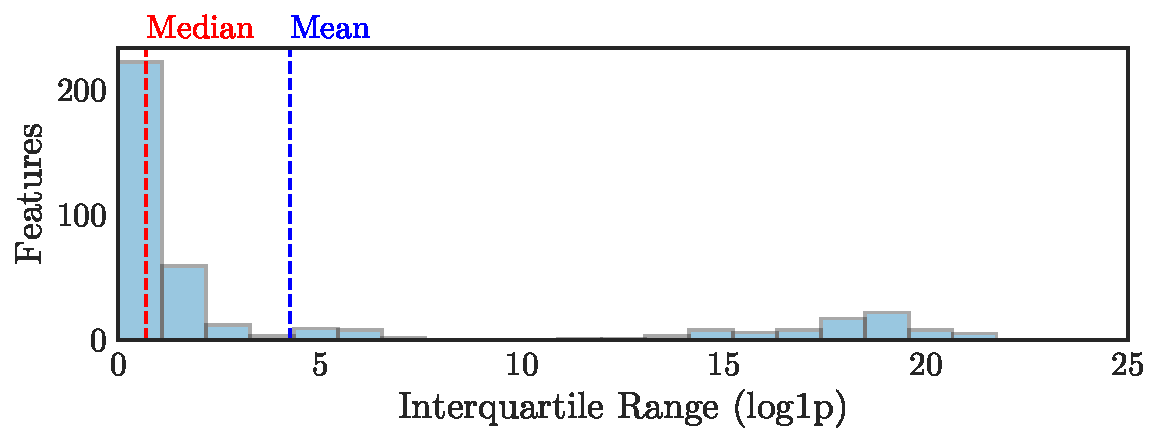
\includegraphics[width=\textwidth]{../figures/design/distribution_ranges}
    \caption[Distribution of interquartile ranges]{Distribution of interquartile ranges (transformed by log1p) in master dataset (c. September 2016).}
    \label{fig:design:scaling}
\end{figure}

\subsubsection{Orthogonality}

Finally, we explored the orthogonality of our features: the extent to which the variance of our features is unrelated. This is a less straight-forward measure. We explore pair-wise inter-correlations between our features and evaluate how many of the inter-correlations are above a particular correlation cut-off, as depicted in Figure~\ref{fig:design:orthogonality}. We use two correlation metrics: Pearson and Spearman. Pearson is more commonly used but Spearman is a ranked metric and may more accurately reflect our non-normal feature distributions. Although most features have relatively low inter-correlations (\~60\% below 0.2) there are still a considerable number that are highly correlated, so it might be efficient to remove these features using an unsupervised feature extractor prior to estimation.

\begin{figure}[!htb]
    \centering
    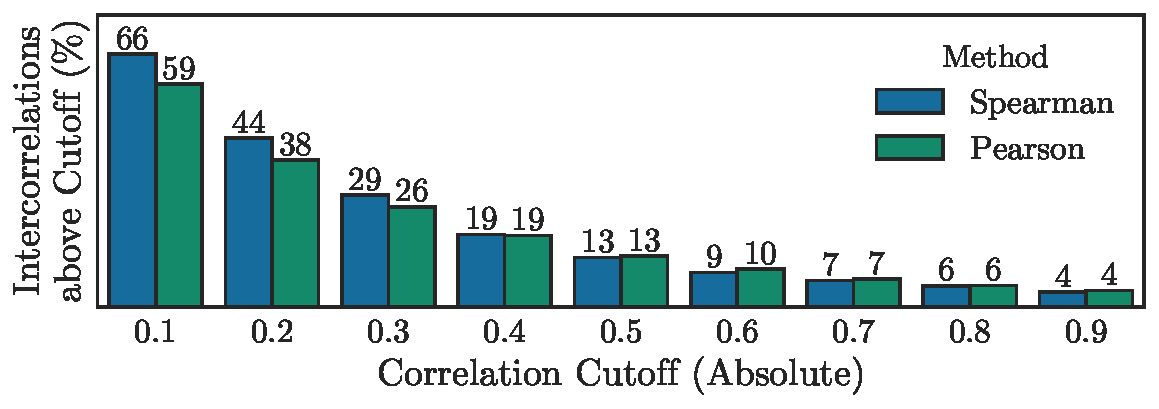
\includegraphics[width=\textwidth]{../figures/design/distribution_orthogonality}
    \caption[Distribution of inter-correlations]{Distribution of inter-correlations.}
    \label{fig:design:orthogonality}
\end{figure}

\section{Pipeline Creation}

We developed a classification pipeline using the popular Python-based machine learning library Scikit-learn \cite{pedregosa2011}. The classification pipeline construct allows us to easily search across hyper-parameters at each step in the pipeline (see Appendix~\ref{appendix:pipeline_hyperparameters} for hyper-parameter list). The following sections explore the testing of each hyper-parameter decision, and the selection of primary classifiers for the following steps. This process is depicted in Figure~\ref{fig:design:pipeline_creation}.

\begin{figure}[!htb]
    \centering
    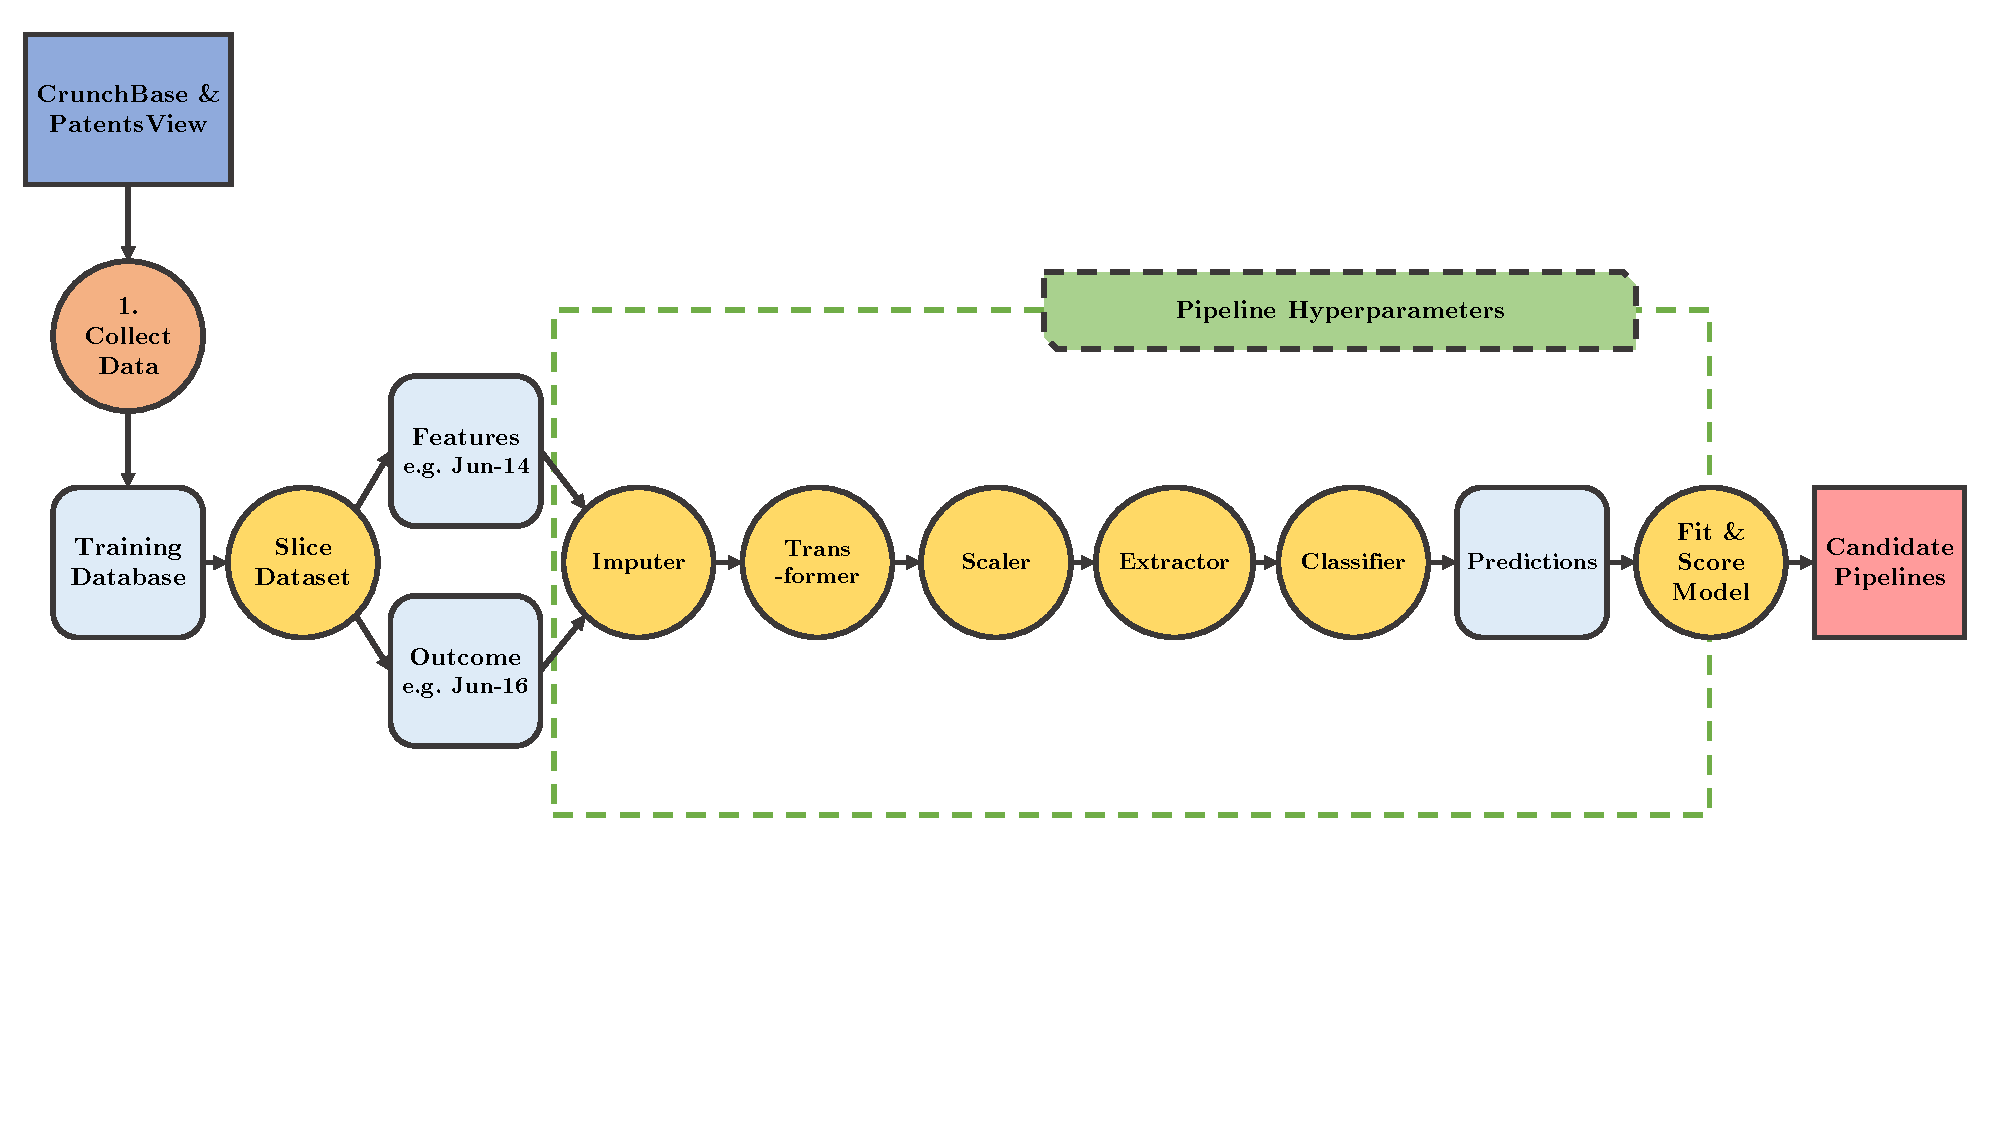
\includegraphics[width=\textwidth]{../figures/design/flowchart_pipeline_creation}
    \caption[Pipeline creation flowchart]{Pipeline creation overview. Legend: dark blue square = input, orange circle = system component, yellow circle = process, light blue rounded square = intermediate, red square = output, green hexagon: iterative process / search space.}
    \label{fig:design:pipeline_creation}
\end{figure}

\subsection{Imputation}

After reviewing the distribution of missing data, we decided to perform further investigation into imputation methods. Common imputation strategies include replacing missing values with the mean, median or mode of each feature. Figure~\ref{fig:design:central_tendency} shows the distribution of mean, median and modes for each feature in the dataset. For the majority of features, all three measures of central tendency are equal to zero. This resolves the issue of distinguishing missing data from negative observations because, following imputation, all of these data points will map to zero. Figure~\ref{fig:design:imputer} shows the receiver-operating characteristics of the different imputation strategies. As expected, all three imputation strategies produce similar results (within the margin of error).

\begin{figure}[!htb]
    \centering
    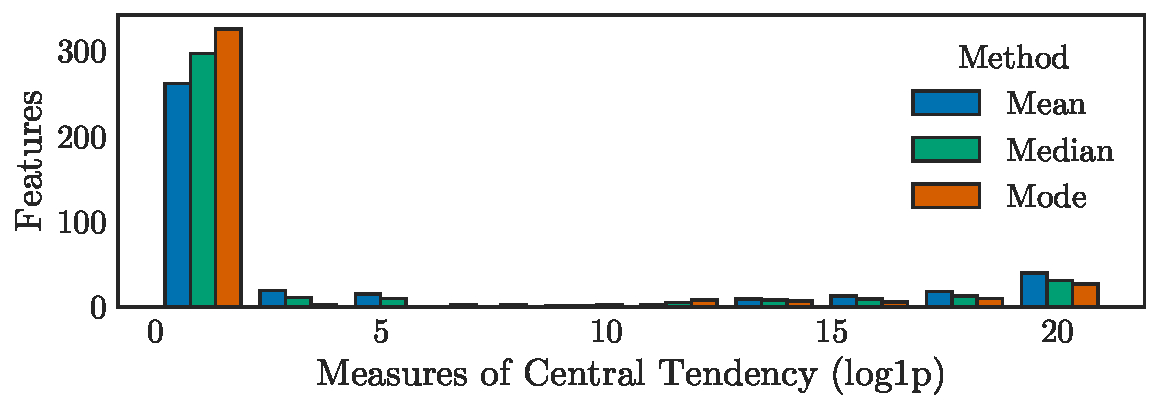
\includegraphics[width=\textwidth]{../figures/design/distribution_central_tendency}
    \caption[Distribution of central tendency]{Distribution of measures of central tendency (mean, median and mode).}
    \label{fig:design:central_tendency}
\end{figure}

\begin{figure}[!htb]
    \centering
    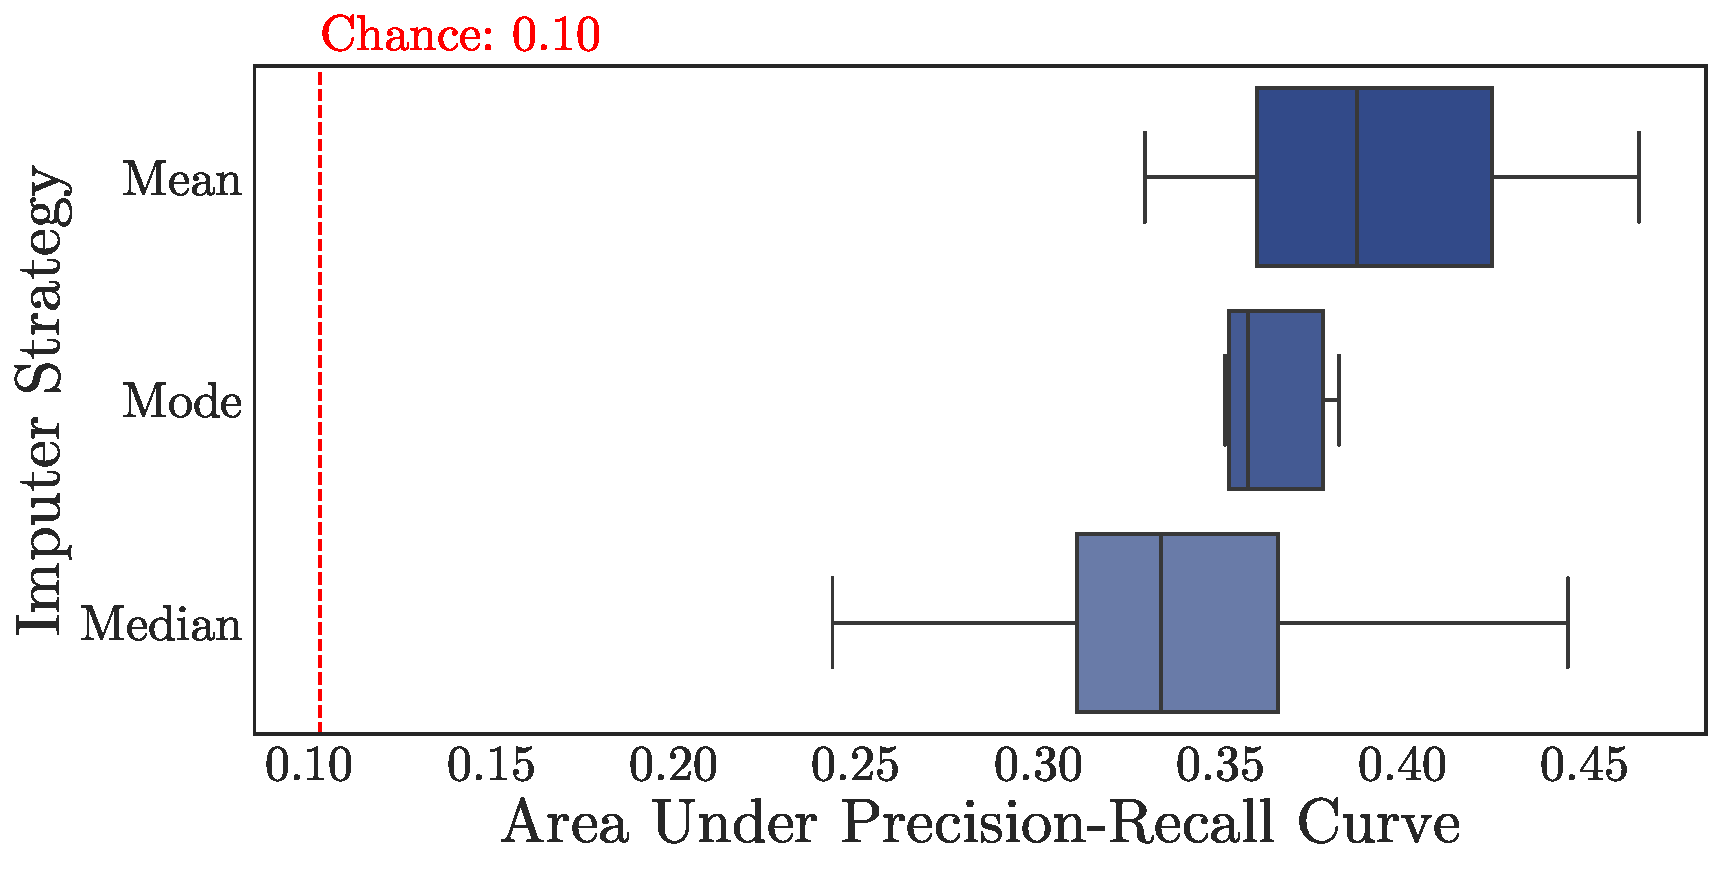
\includegraphics[width=\textwidth]{../figures/design/auc_imputer}
    \caption[Area under PR Curves by imputation strategy]{Area under \gls{roc} for different imputation strategies. Imputation strategies include replacing missing values with the most frequent (mode), median and mean value of each respective feature. Results presented are aggregated from hyper-parameter optimisation performed over entire classification pipeline (including all classifiers). Source: Features (Apr-12) and labels (Apr-14, 2 year forecast window) derived from Master dataset (c. Sep-16).}
    \label{fig:design:imputer}
\end{figure}

\subsection{Transformation}

While the classification algorithms we identified in the previous chapter are relatively robust to violations of normality, it may be beneficial to transform the data if the feature distributions are extreme. Figure~\ref{fig:design:funding_transformation} shows one of the key features, Total Funding Raised, under a number of different transformations. Like many features in our dataset, the distribution of Total Funding Raised is highly skewed. The log transformation reduces this skewness (a normal distribution of non-zero values becomes visible) and square root transformation also reduces this skewness (to a lesser extent). The impact of these transformations is reduced by the extent of their zero-inflation. However, it is still reasonable to expect both of these transformations to improve the classification accuracy. Figure~\ref{fig:design:transformer} shows the \gls{roc} of these different transformation functions. Both functions provide a small performance improvement, with the square root function narrowly best.

\begin{figure}[!htb]
    \centering
    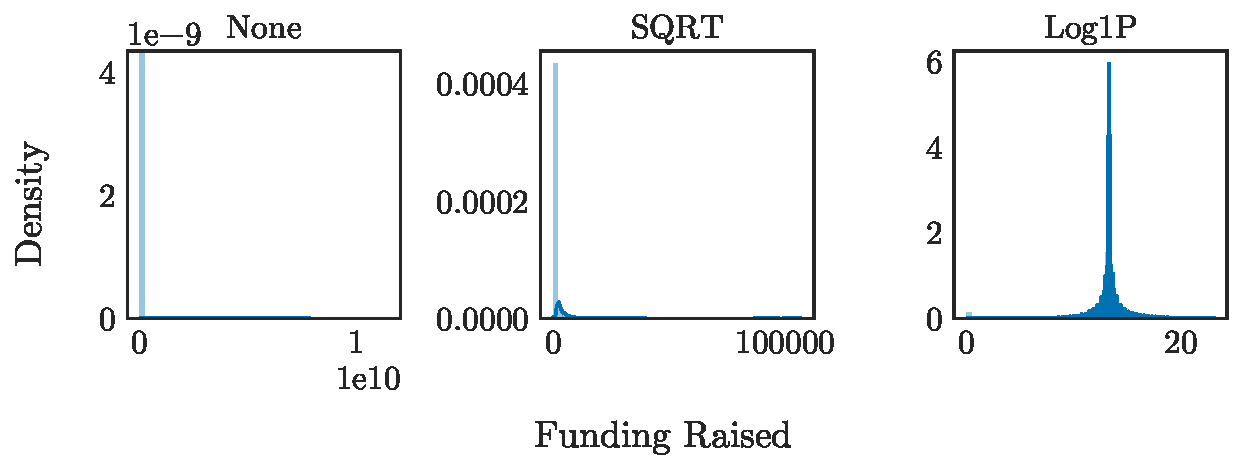
\includegraphics[width=\textwidth]{../figures/design/distribution_funding_transformed}
    \caption[Funding raised transformed by functions]{Funding raised transformed by functions.}
    \label{fig:design:funding_transformation}
\end{figure}

\begin{figure}[!htb]
    \centering
    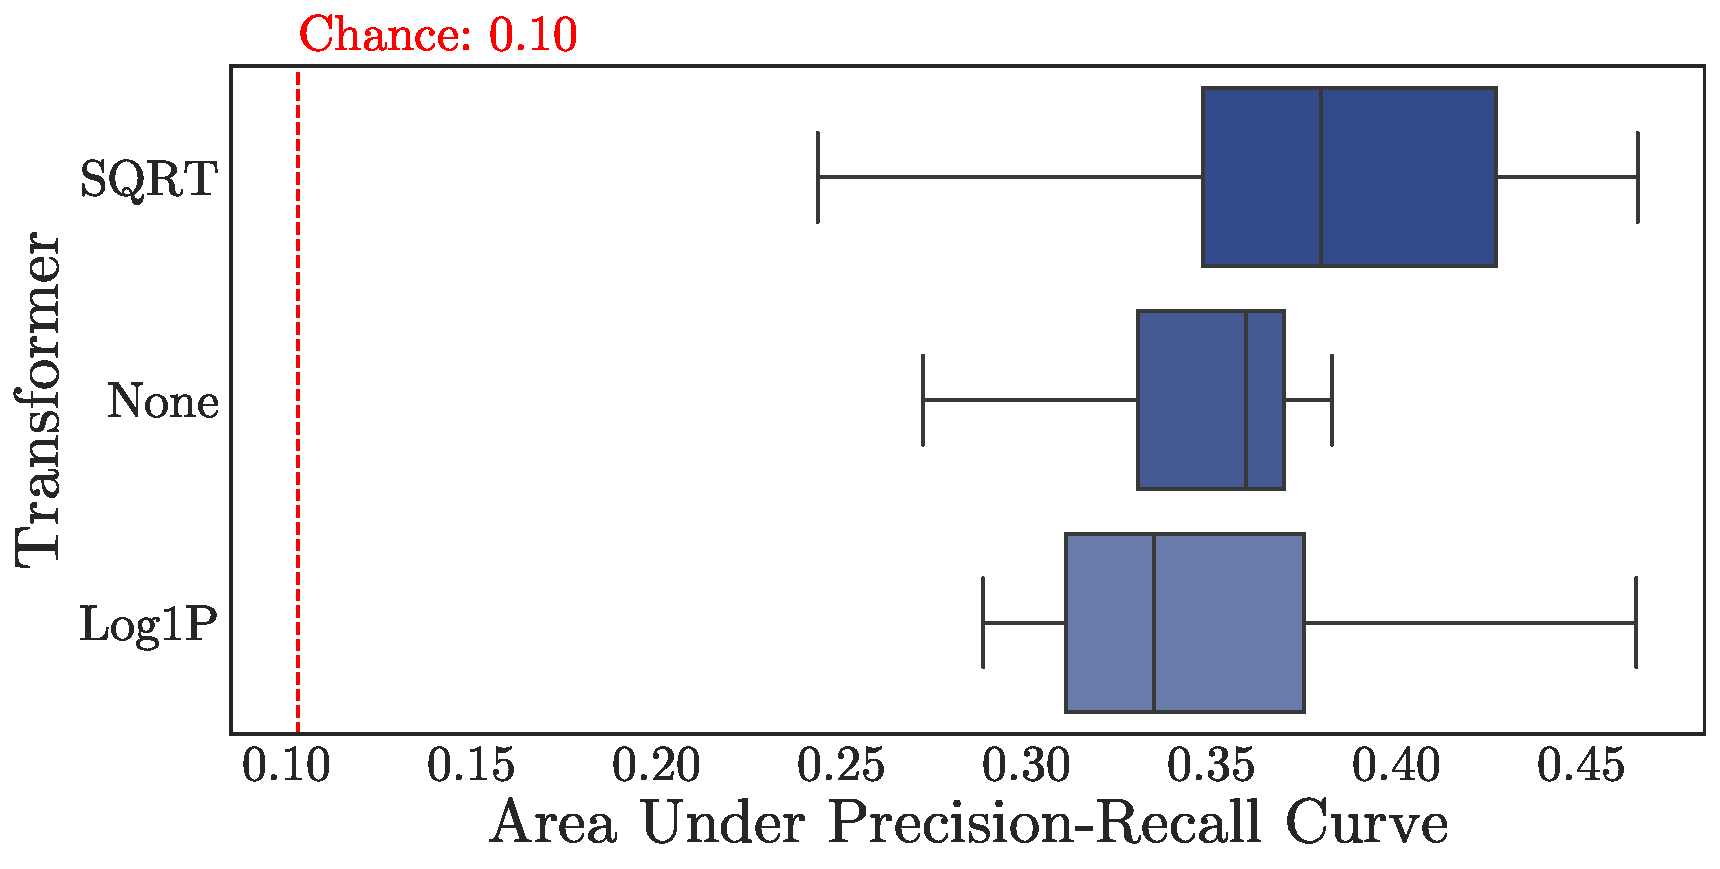
\includegraphics[width=\textwidth]{../figures/design/auc_transformer}
    \caption[Area under PR Curves by transformation function]{Area under \gls{roc} for different transformation functions. Transformations include: None (identity transformation), Log1p (natural logarithm of one plus the input array, element-wise), and Sqrt (the square root of the input array, element-wise). Results presented are aggregated from hyper-parameter optimisation performed over entire classification pipeline (including all classifiers).Source: Features (Apr-12) and labels (Apr-14, 2 year forecast window) derived from Master dataset (c. Sep-16).}
    \label{fig:design:transformer}
\end{figure}

\subsection{Scaling}

Standardisation of datasets is a common requirement for many feature extraction methods and machine learning estimators. Sci-kit learn provides three primary scaling functions: StandardScaler, RobustScaler and MinMaxScaler. RobustScaler is intended to alleviate the effect of outliers while MinMaxScaler is intended to preserve zero entries in sparse data - both of these are relevant properties for the dataset. Figure~\ref{fig:design:scaler} shows the receiver-operating characteristics of the different scaling functions. MinMaxScaler and RobustScaler actually under-perform the null condition while StandardScaler only performs on par with the null condition. This is unexpected but may be caused by the previously applied transformations.

\begin{figure}[!htb]
    \centering
    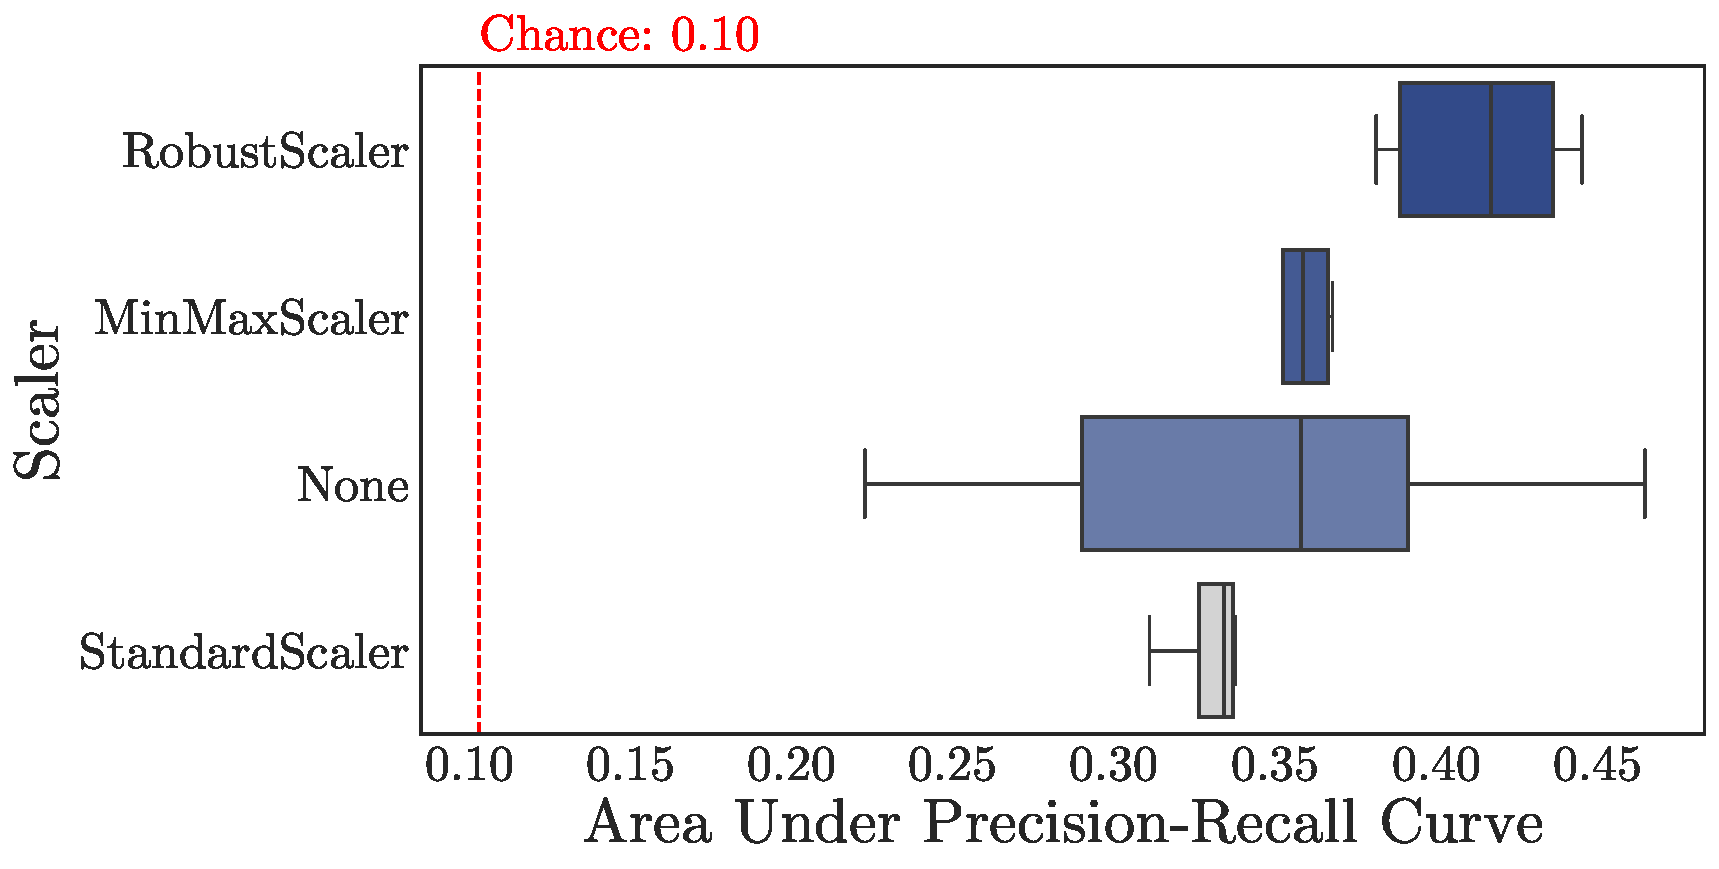
\includegraphics[width=\textwidth]{../figures/design/auc_scaler}
    \caption[Area under PR Curves by scaling function]{Area under \gls{roc} for different scaling functions. Scaling functions include: None, StandardScaler (mean: 0, variance: 1), RobustScaler (median: 0, IQR: 1) and MinMaxScaler (min: 0, max: 1). Results presented are aggregated from hyper-parameter optimisation performed over entire classification pipeline (including all classifiers).Source: Features (Apr-12) and labels (Apr-14, 2 year forecast window) derived from Master dataset (c. Sep-16).}
    \label{fig:design:scaler}
\end{figure}

\subsection{Extraction}

Feature extraction reduces high-dimensional data into lower-dimensional data in such a way that maximises the variance of the data. The most common approach to dimensionality reduction is \gls{pca}. \Gls{pca} is a technique which takes a set of vectors and finds an uncorrelated coordinate system in which to represent these vectors \cite{jolliffe2002}. This new co-ordinate system optimally distributes the variance, so that the first basis vector (eigenvector) has the largest possible variance and all successive eigenvector have the largest possible variance given that they are strictly uncorrelated with the previous eigenvectors. The magnitude of each eigenvector (its eigenvalue) is displayed in Figure~\ref{fig:design:scree_plot}. The majority of explained variance is captured in the first 10 components, and the eigenvalues drop below 1 by 100 components - this suggests that these are reasonable values for further hyper-parameter search. Figure~\ref{fig:design:extractor} shows the \gls{roc} for different numbers of extracted components. All curves produce similar classification results (within margin of error) which implies that we should extract between 1 -- 20 components because it will provide us with more efficient computation.

\begin{figure}[!htb]
    \centering
    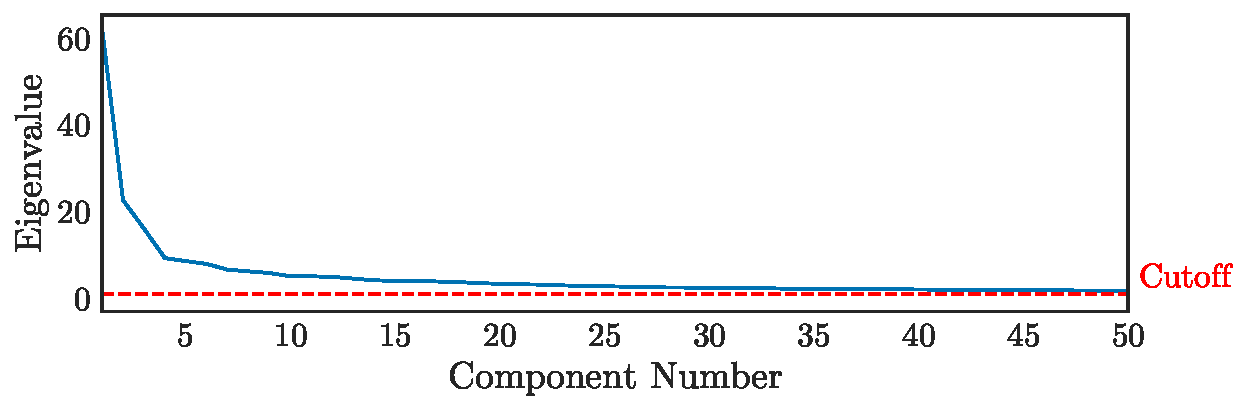
\includegraphics[width=\textwidth]{../figures/design/distribution_eigenvalues}
    \caption[PCA scree plot]{Eigenvalues extracted from \gls{pca} model. Horizontal line drawn at an Eigenvalue of 1 -- this theoretically represents the `contribution' of one original feature and is commonly used as an approximate threshold for included components. Source: Master dataset (c. Sep-2016).}
    \label{fig:design:scree_plot}
\end{figure}

\begin{figure}[!htb]
    \centering
    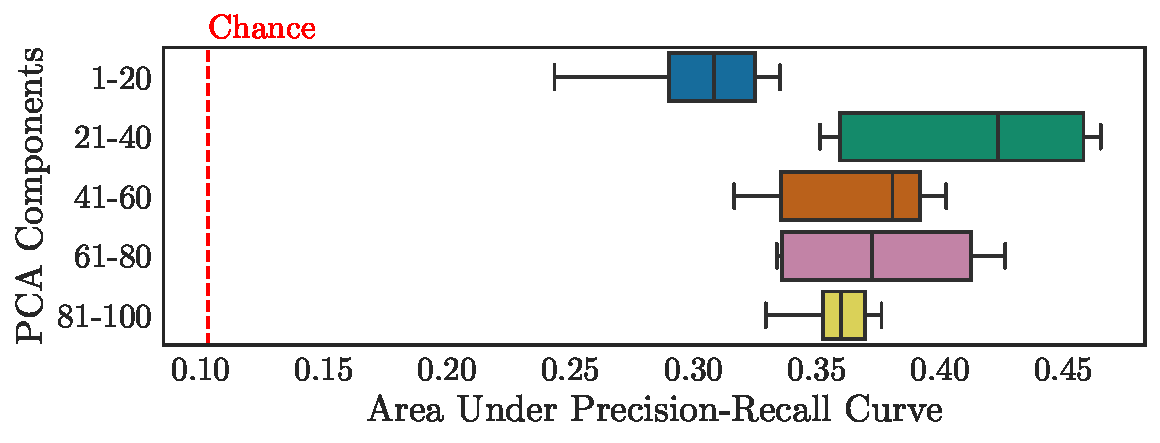
\includegraphics[width=\textwidth]{../figures/design/auc_extractor}
    \caption[Area under PR Curves by PCA techniques]{Area under \gls{roc} for different number of extracted components from \gls{pca}. Curves have been grouped by the quotient of the number of components divided by 20 to result in five ordered groups (e.g. Range [0, 19] becomes 0). Results presented are aggregated from hyper-parameter optimisation performed over entire classification pipeline (including all classifiers).Source: Features (Apr-12) and labels (Apr-14, 2 year forecast window) derived from Master dataset (c. Sep-16).}
    \label{fig:design:extractor}
\end{figure}

While \gls{pca} is efficient at reducing features, the resultant components are not interpretable. Similarly, individual analysis of 400+ features is difficult to interpret. A compromise is to group the features using the conceptual framework we developed earlier from the literature review. The grouping approach applied weights to each individual feature that optimised the inter-correlations within each group. Given the highly skewed features, we use Spearman correlation which is robust to skewness because it is based on ranking. Figure~\ref{fig:design:grouped_heatmap} displays the inter-correlations between each factor from the conceptual framework. As we would expect, Investors and Funding features are highly correlated. While Investors captures the influence of previous investors, it also captures features like the size of an investor's past investments, which would likely correlate with the size of the investment they made in the target company. Interestingly, Founders features are positively correlated with all other features except for Advisors features which are negatively correlated with all other feature groups.

\begin{figure}[!htb]
    \centering
    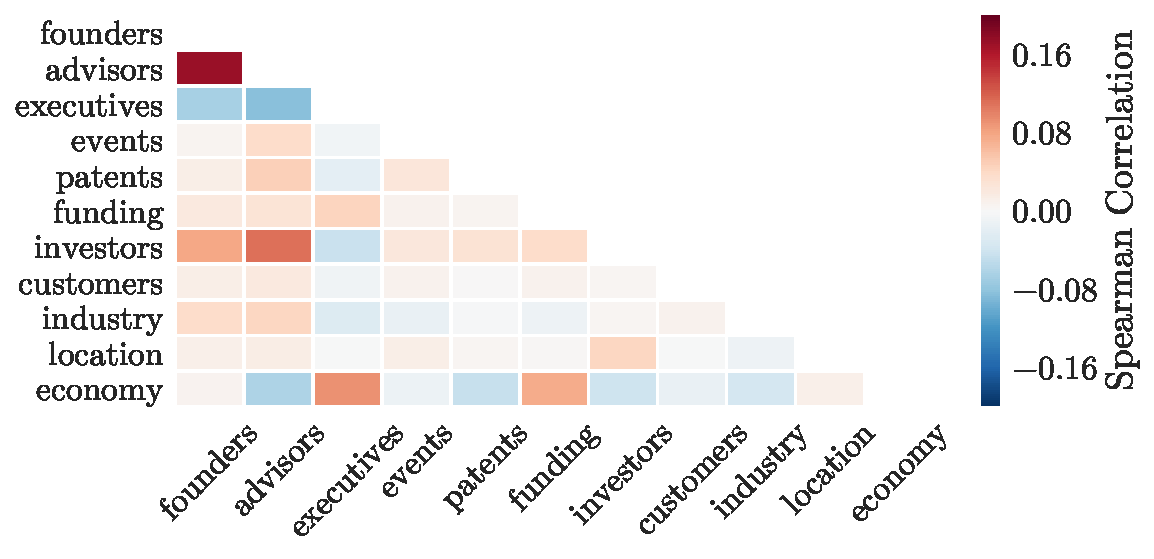
\includegraphics[width=\textwidth]{../figures/design/distribution_correlations_grouped}
    \caption[Inter-correlations of factors from framework]{Inter-correlations of each factor from conceptual framework. Spearman ranking correlation is used. Individual features are grouped by applying weights that maximise the inter-correlations within each group from our conceptual framework (see Figure~\ref{fig:design:features:framework_simple}). Source: Master dataset (c. Sep-2016).}
    \label{fig:design:grouped_heatmap}
\end{figure}

\subsection{Classification Algorithms}

The literature review we performed in the previous chapter revealed seven common supervised classification algorithms potentially suitable for application to this problem area. Our review suggested that Random Forests were most likely to provide a successful trade-off between predictive power, interpretability and time taken. We empirically tested each of these classifiers and compared their performance against a range of metrics, as displayed in Table~\ref{fig:design:classification_metrics}. We report maximum as well as median recorded scores to ensure we didn't penalise algorithms that had unfavourable hyper-parameter search spaces.

\begin{table}[!htb]
    \centering
    \scalebox{0.8}{\begin{tabular}{lrrrrrrrrrr}
\toprule
{} & \multicolumn{2}{c}{AUC PRC}        & \multicolumn{2}{c}{AUC ROC}        &     \multicolumn{2}{c}{F1}       &    \multicolumn{2}{c}{MCC}        & \multicolumn{2}{c}{Fit Time (s)}         \\
{Classifier} &    Median &    Max &    Median &    Max &   Median &    Max &   Median &    Max &         Median &     75th \\
\midrule
LR       &   0.417 &  0.465 &   0.675 &  0.710 &  0.339 &  0.358 &  0.255 &  0.288 &        7.3 &  412.7 \\
RF             &   0.376 &  0.465 &   0.619 &  0.709 &  0.332 &  0.360 &  0.271 &  0.288 &       68.3 &   69.0 \\
DT             &   0.388 &  0.429 &   0.651 &  0.659 &  0.305 &  0.314 &  0.212 &  0.224 &       15.3 &   16.8 \\
NB               &   0.354 &  0.367 &   0.623 &  0.638 &  0.303 &  0.321 &  0.212 &  0.239 &        8.6 &   26.8 \\
KNN       &   0.335 &  0.353 &   0.532 &  0.565 &  0.131 &  0.226 &  0.137 &  0.210 &        8.5 &   20.8 \\
ANN &   0.320 &  0.335 &   0.517 &  0.523 &  0.072 &  0.096 &  0.111 &  0.140 &        9.1 &   21.0 \\
SVM    &   0.233 &  0.244 &   0.503 &  0.504 &  0.014 &  0.017 &  0.038 &  0.045 &       29.0 &   29.0 \\
Total                     &   0.357 &  0.465 &   0.623 &  0.710 &  0.300 &  0.360 &  0.209 &  0.288 &       15.3 &   29.0 \\
\bottomrule
\end{tabular}
}
    \caption[Overview of classification algorithm performance]{Overview of classification algorithm performance.}
    \label{fig:design:classification_metrics}
\end{table}

We take a closer look at the \gls{pr} curves for each classifier in Figure~\ref{fig:design:classifier}. While all classifiers perform better than chance, Logistic Regressions and Random Forests come out ahead, and Support Vector Machines and Artificial Neural Networks appear to under-perform. Delving into the cross-validated learning curves for each classifier (Figure~\ref{fig:design:create_learning_curves}) we see that Naive Bayes, Logistic Regression, Artificial Neural Networks and Support Vector Machines quickly converge, whereas Decision Trees, Random Forests and K-Nearest Neighbours require more observations to converge. This suggests that we might expect Random Forests to do better in final testing (as testing will not be cross-validated), as well as in the future as the dataset naturally grows.

\begin{figure}[!htb]
    \centering
    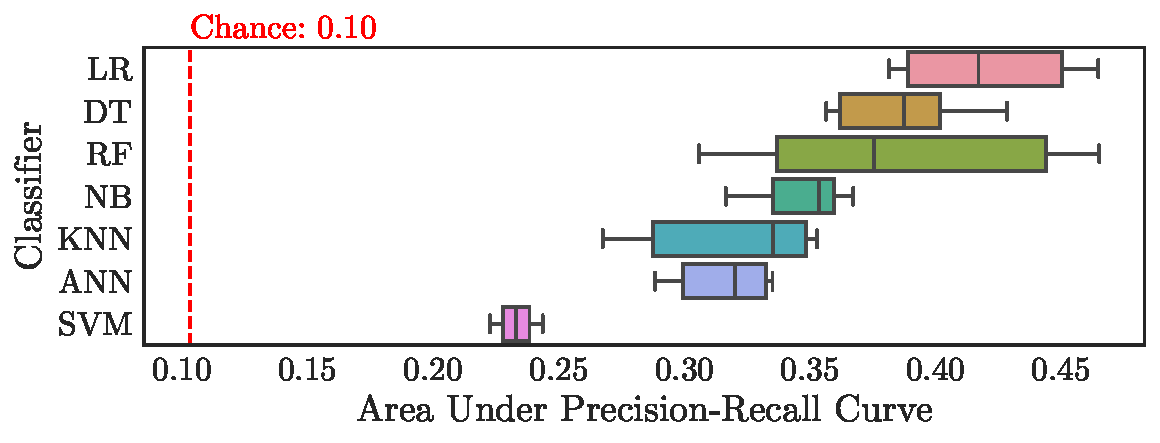
\includegraphics[width=\textwidth]{../figures/design/auc_classifier}
    \caption[Area under PR Curves by classification algorithms]{Area under \gls{roc} for different classification algorithms. All algorithms are implementations from the Sci-kit learn library. Results presented are aggregated from hyper-parameter optimisation performed over entire classification pipeline (including all classifiers).Source: Features (Apr-12) and labels (Apr-14, 2 year forecast window) derived from Master dataset (c. Sep-16).}
    \label{fig:design:classifier}
\end{figure}

\begin{figure}[!htb]
    \centering
    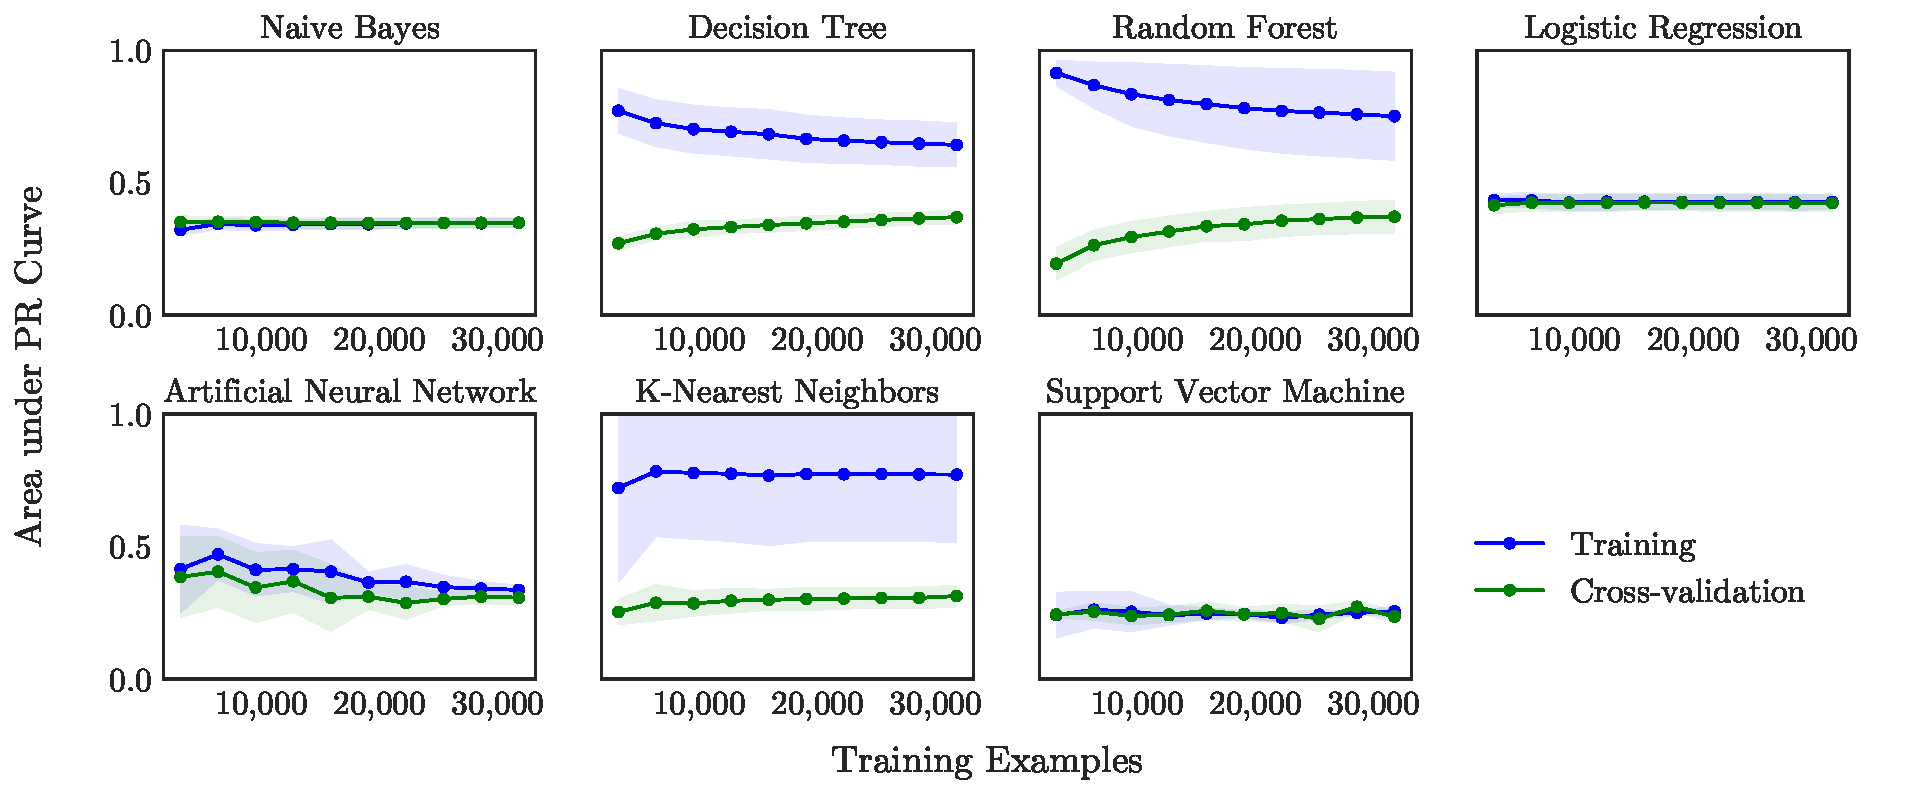
\includegraphics[width=\textwidth]{../figures/design/learning_curves_classifier}
    \caption[Learning curves by classification algorithms]{Learning curves by classification algorithms.}
    \label{fig:design:create_learning_curves}
\end{figure}

\section{Pipeline Selection}

In the previous chapter, we developed a system that generated a cross-section of candidate pipelines with different hyper-parameters. In this step, we rank these candidate pipelines and evaluate the best pipelines (finalist pipelines) over a number of different dataset slices. This process, depicted in Figure~\ref{fig:design:pipeline_selection}, ensures that our final pipeline is robust in their performance with respect to time. We aggregate the results for each finalist pipeline across these dataset slices and rank the finalist pipelines on their overall performance. Finally, we select the best pipeline.

\begin{figure}[!htb]
    \centering
    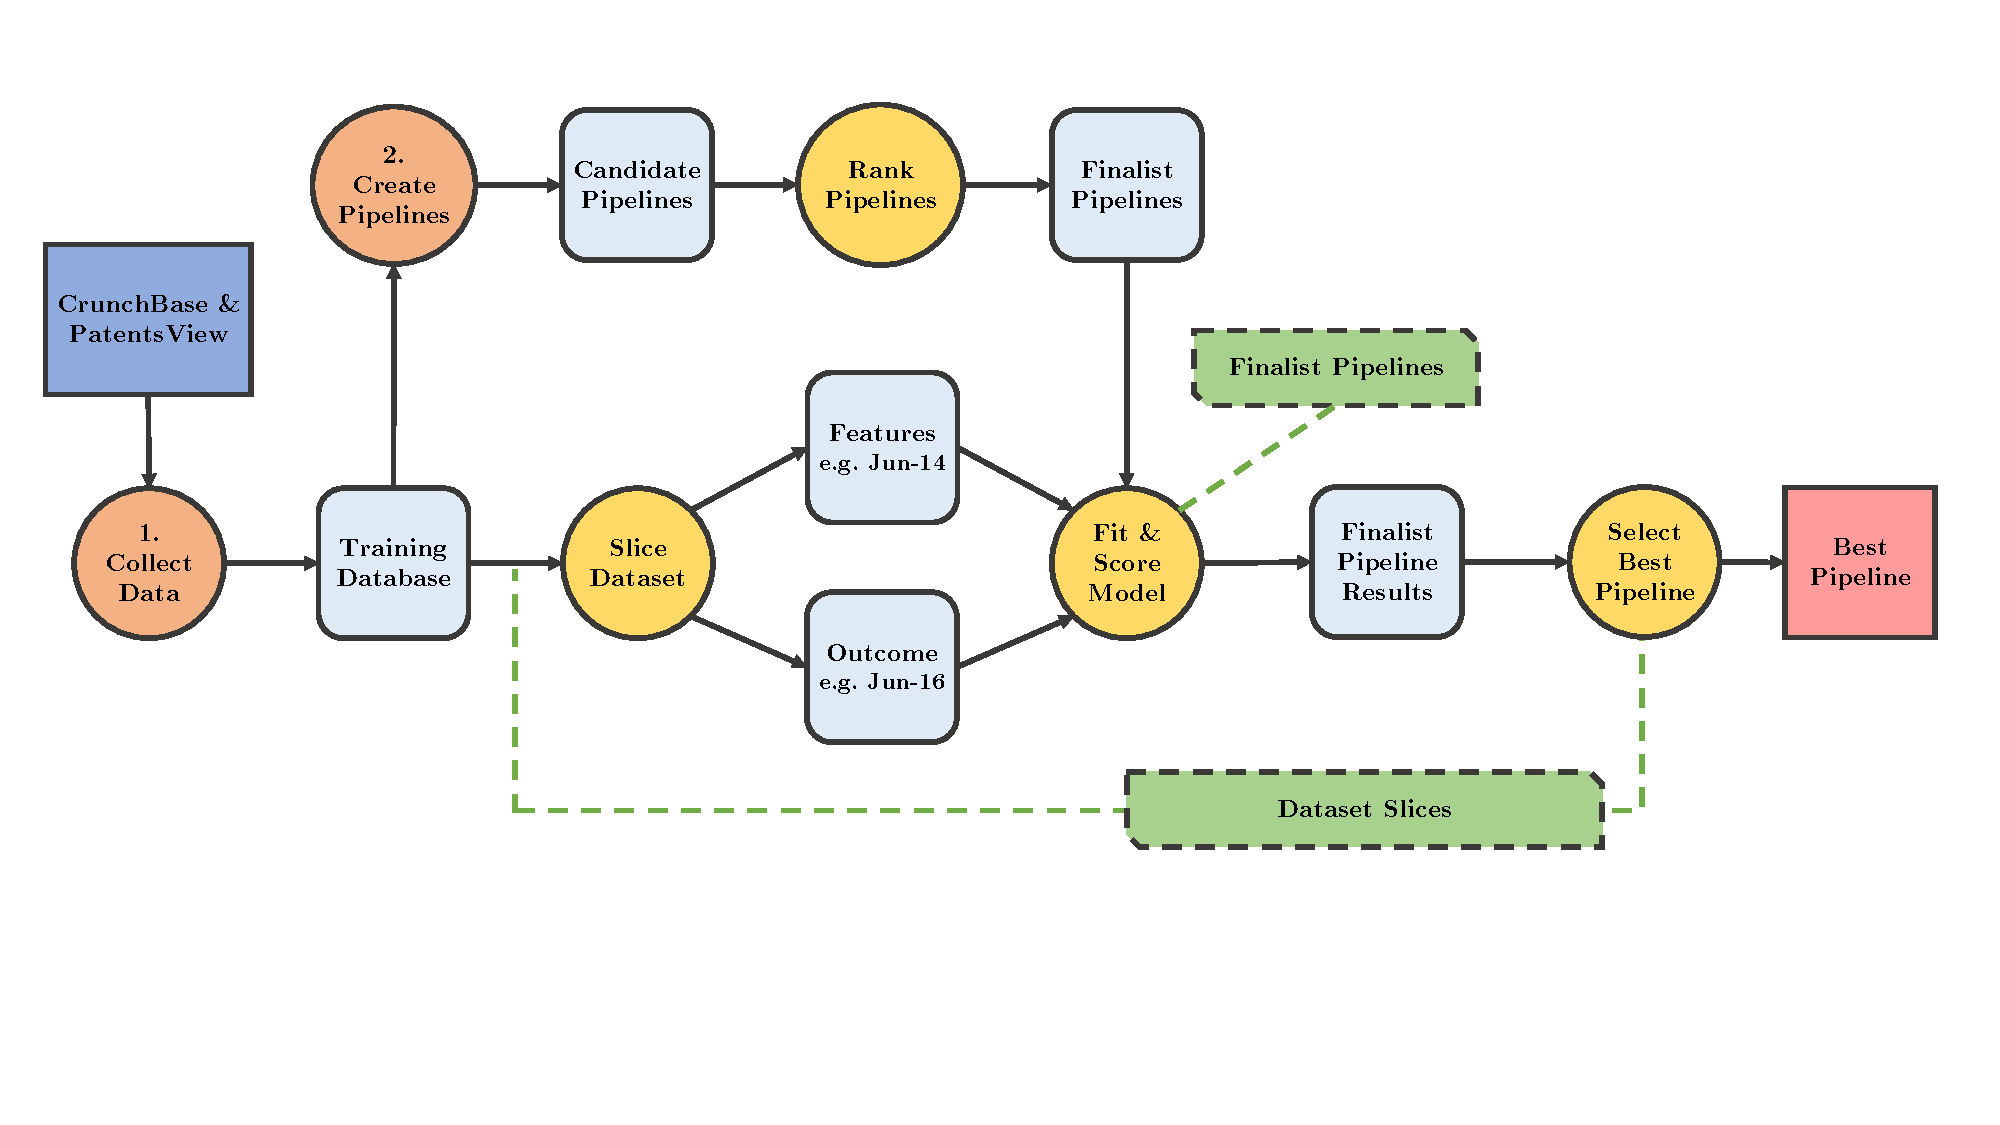
\includegraphics[width=\textwidth]{../figures/design/flowchart_pipeline_selection}
    \caption[Pipeline selection flowchart]{Pipeline selection overview. Legend: dark blue square = input, orange circle = system component, yellow circle = process, light blue rounded square = intermediate, red square = output, green hexagon: iterative process / search space.}
    \label{fig:design:pipeline_selection}
\end{figure}

\subsection{Dataset Slicing}

We developed a procedure for generating historical datasets from our CrunchBase and PatentsView data. CrunchBase provides created and last-updated timestamps for each record in their CSV-formatted dumps (and also in the JSON-formatted responses from their API). We took advantage of this to produce a system that reverse-engineers previous database states by filtering the current database by only records that were created by a given 'slice' date.

We performed preliminary testing of our reverse-engineering technique by comparing a historical CrunchBase database collected in December 2013 with a slice from our primary dataset collected in September 2016, as shown in Figure~\ref{fig:design:counts_slice_method}. While there are some differences, particularly in the IPO counts, we consider this to be satisfactory variance considering the 3-year time difference (i.e. perhaps some companies have been since removed from the database). The key relations for the purposes of our system are Companies, Funding Rounds and People, all of which had minor differences considering the size of these datasets.

\begin{figure}[!htb]
    \centering
    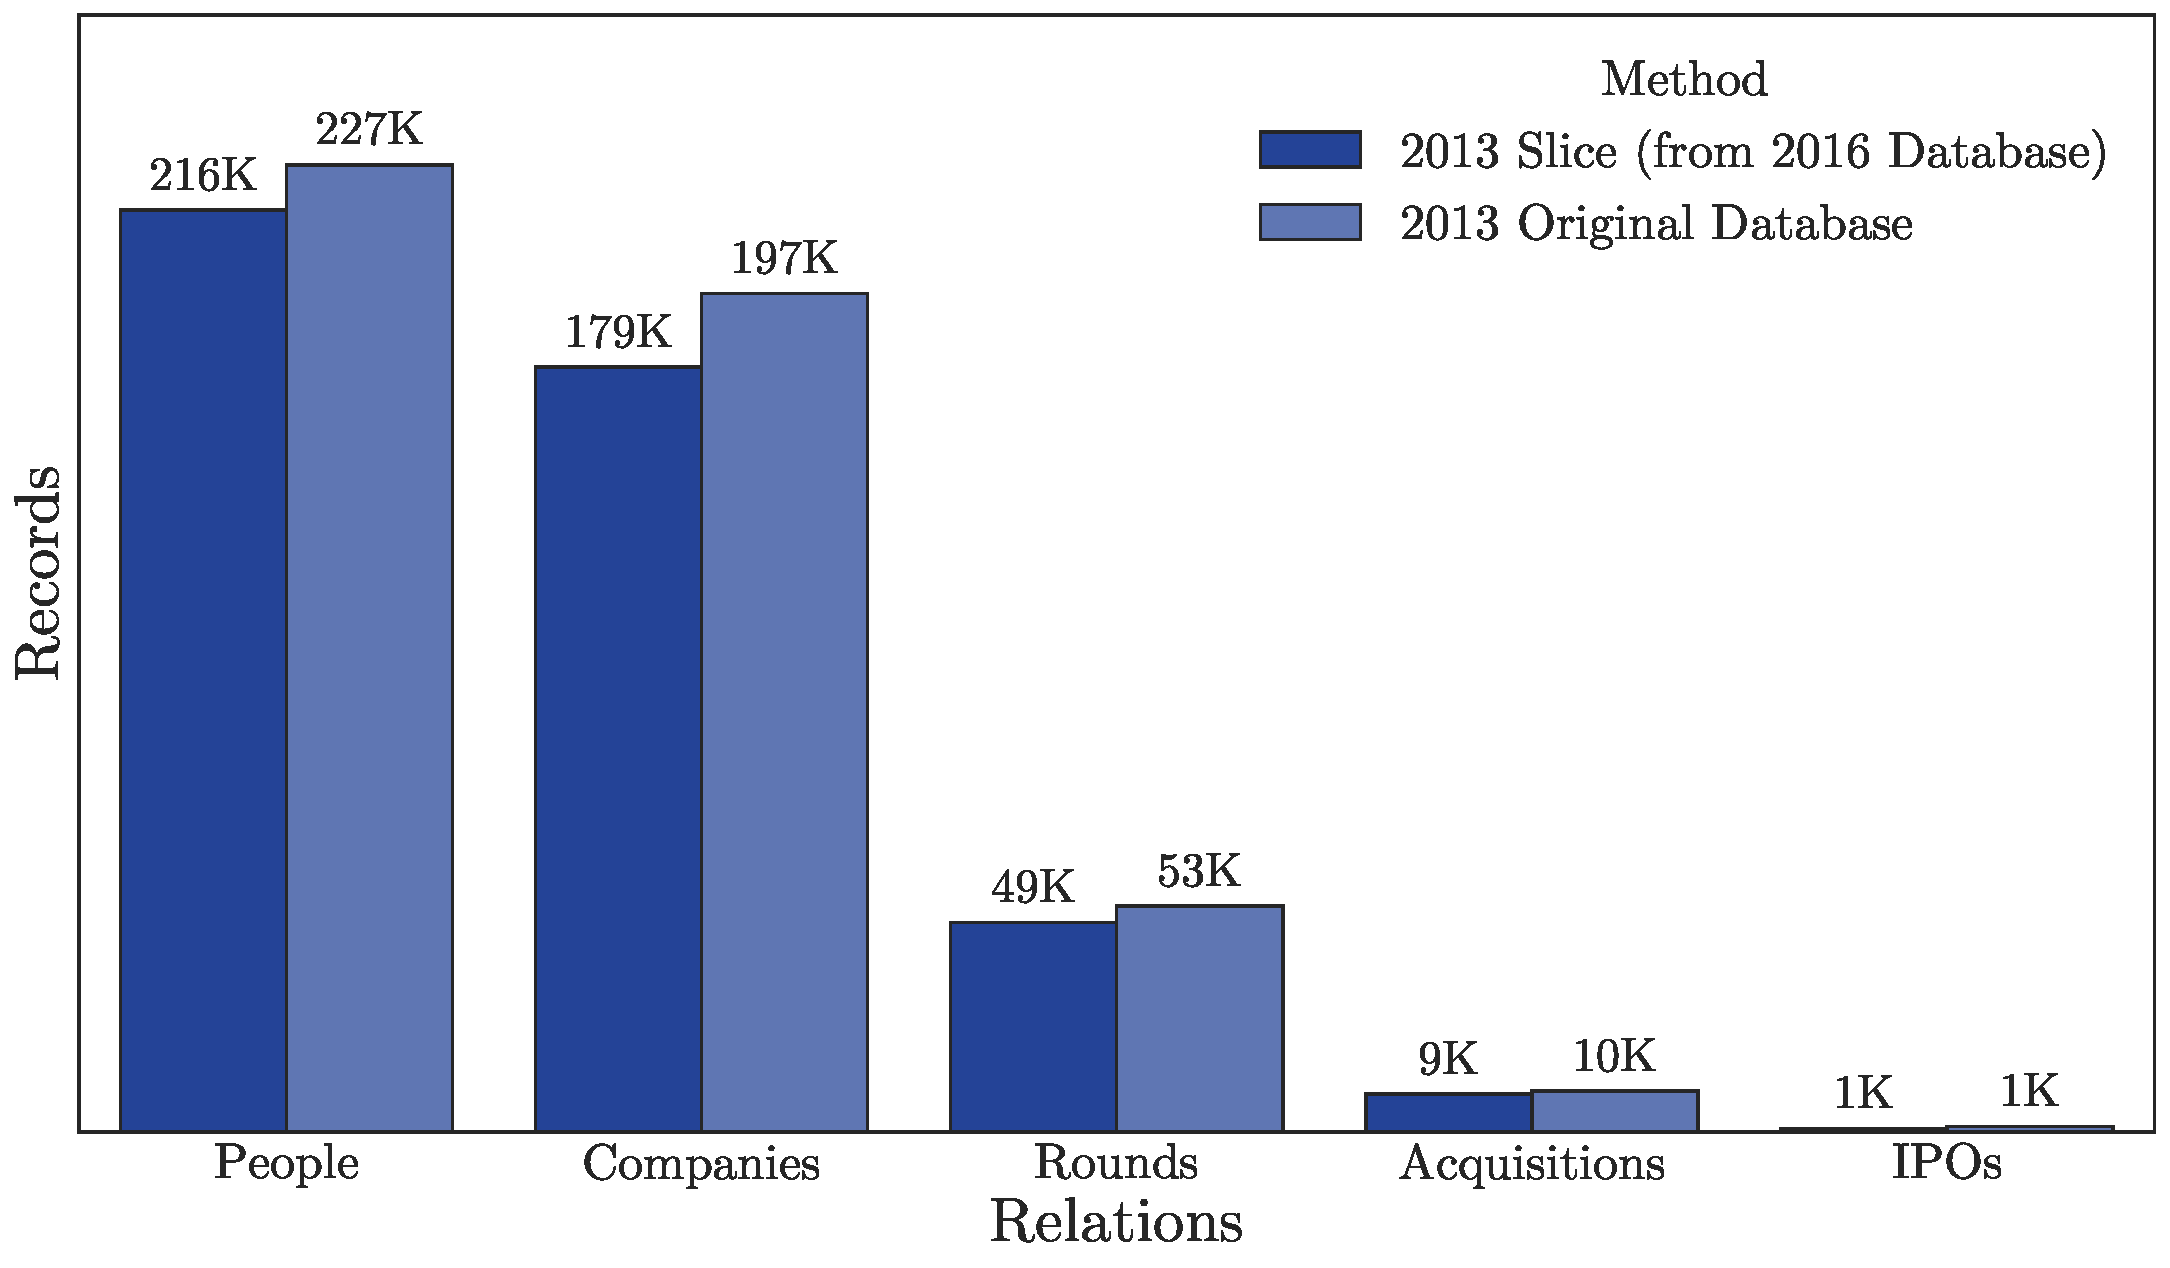
\includegraphics[width=\textwidth]{../figures/design/counts_slice_method}
    \caption[Dataset slice compared with original database]{Dataset slice compared with original dataset.}
    \label{fig:design:counts_slice_method}
\end{figure}

Figure~\ref{fig:design:slice_counts_over_time} shows company counts by startup development stage from different dataset slices. We limited our experiments to dataset slices from 2012-onwards because prior to 2012 the datasets become too small to use to make predictions (particularly given the class imbalance).

\begin{figure}[!htb]
    \centering
    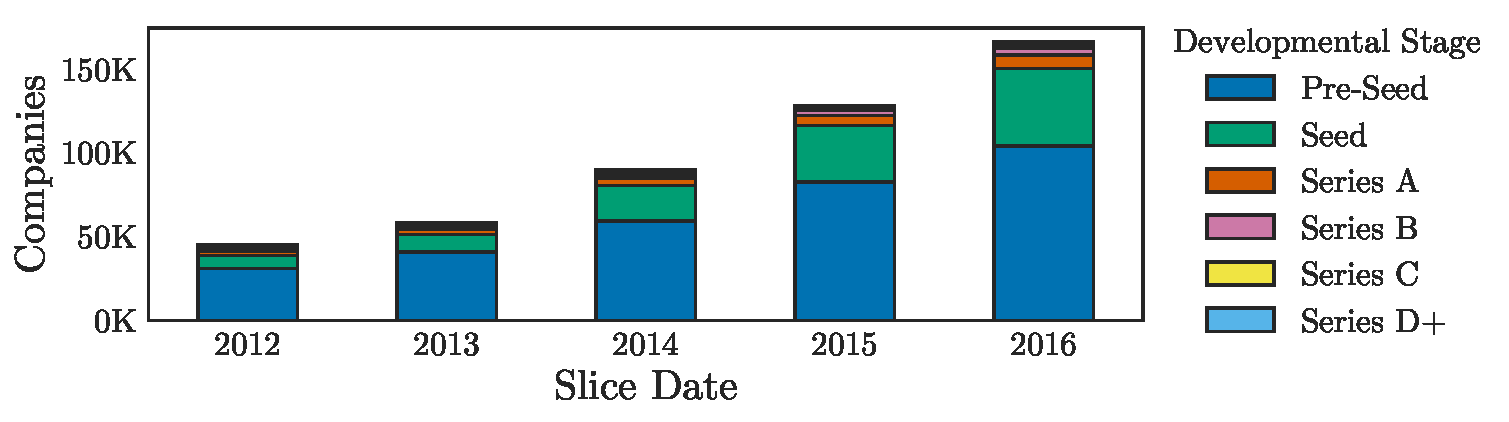
\includegraphics[width=\textwidth]{../figures/design/counts_stage_slice}
    \caption[Dataset counts over time]{Dataset slice counts over time.}
    \label{fig:design:slice_counts_over_time}
\end{figure}

\subsection{Evaluation Metrics}

Next, we decided how to narrow our candidate pipelines down to finalist pipelines that we can evaluate further. There are a number of different metrics used to evaluate binary classifiers in machine learning. The most simplistic metric is accuracy but this is rarely used in practice because it gives misleading results in the case of imbalanced classes. \Gls{roc} curves are perhaps the mostly commonly used evaluation tool in binary classification, and show how the number of correctly classified positive examples varies with the number of incorrectly classified negative examples. The area under these curves gives a standardised result across a spectrum of decision thresholds. \Gls{pr} curves are similar to \gls{roc} curves but instead map the trade-offs between precision and recall. They are less commonly used than \gls{roc} curves but have been shown to produce more accurate results for imbalanced classes than \gls{roc} curves \cite{davis2006}. Given our dataset is highly imbalanced (the positive class is approximately 10\%) we decided to proceed with \gls{pr} curves. We will also use this metric to determine which is ultimately the best of our finalist pipelines.

\subsection{Finalist Pipeline Evaluation}

Our hypothesis is that the performance of our classification pipelines may vary with respect to the date that the dataset was collected (in this case, sliced). To study this hypothesis, first we explored variance between the pipelines on aggregate against the slice dates, presented in Figure~\ref{fig:design:selection_agg_slice}. We see little variance on this basis, and we don't observe a relationship between slice date and score.

\begin{figure}[!htb]
    \centering
    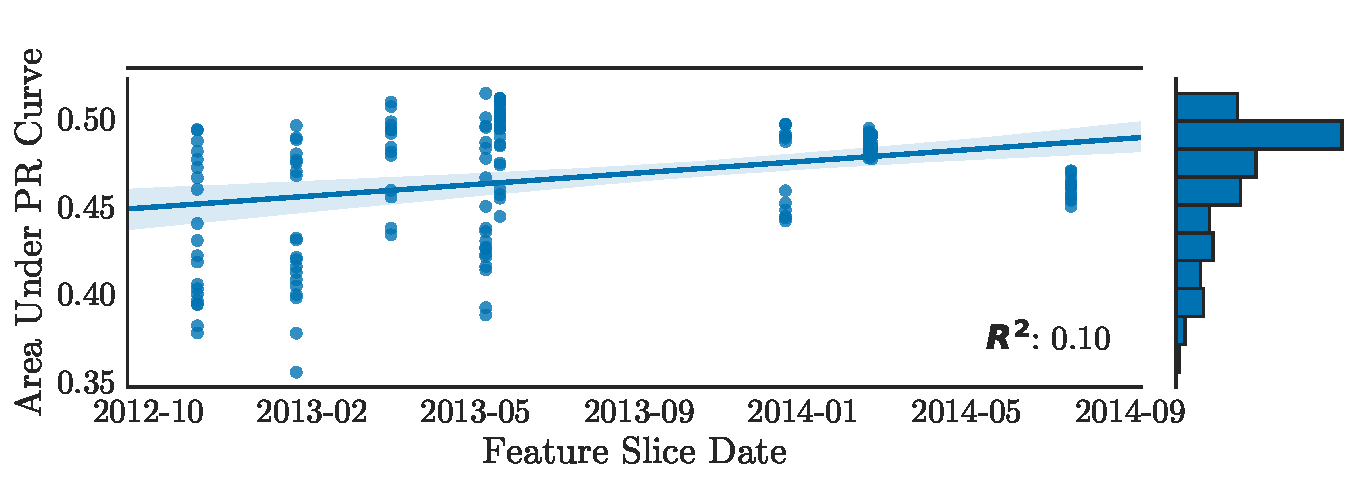
\includegraphics[width=\textwidth]{../figures/design/auc_finalists_agg}
    \caption[Pipeline performance by slice date]{Pipeline performance by slice date.}
    \label{fig:design:selection_agg_slice}
\end{figure}

Next, we study the variance within the individual pipelines, presented in Figure~\ref{fig:design:selection_agg_rank}. Here, we can see there is significantly more variance in the scores. Although there is still a strong positive correlation between the pipelines initial ranking and their scores, we can see that there are some individual deviations. Importantly, the top-ranked pipeline from the first stage actually has a lower median score than the second-ranked pipeline. These results suggest that the top 3-5 pipelines should be evaluated in this manner to ensure that the best pipeline is selected. The candidate pipeline selected by this process is depicted in Table~\ref{appendix:experimental_config}. We adopted this pipeline configuration for our following experiments.

\begin{figure}[!htb]
    \centering
    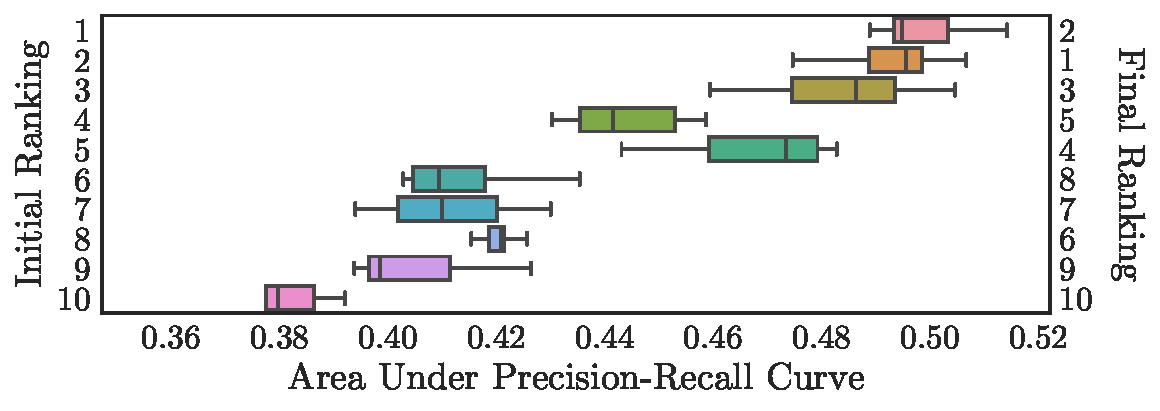
\includegraphics[width=\textwidth]{../figures/design/auc_finalists_rank}
    \caption[Overview of finalist pipeline performance]{Overview of finalist pipeline performance.}
    \label{fig:design:selection_agg_rank}
\end{figure}

\section{Model Fit and Prediction}

Finally, we use our optimised pipeline to estimate a model and make predictions, as shown in Figure~\ref{fig:design:make_predictions}. Our system applies the best pipeline that was generated in the previous section to a training dataset, producing a fitted model. The model is then applied to a feature vector from a held-out test database, which generates a set of predictions which could, in practice, then be used by \gls{vc} firms. We evaluate the accuracy of the models produced by our system with respect to a number of variables in the next chapter.

\begin{figure}[!htb]
    \centering
    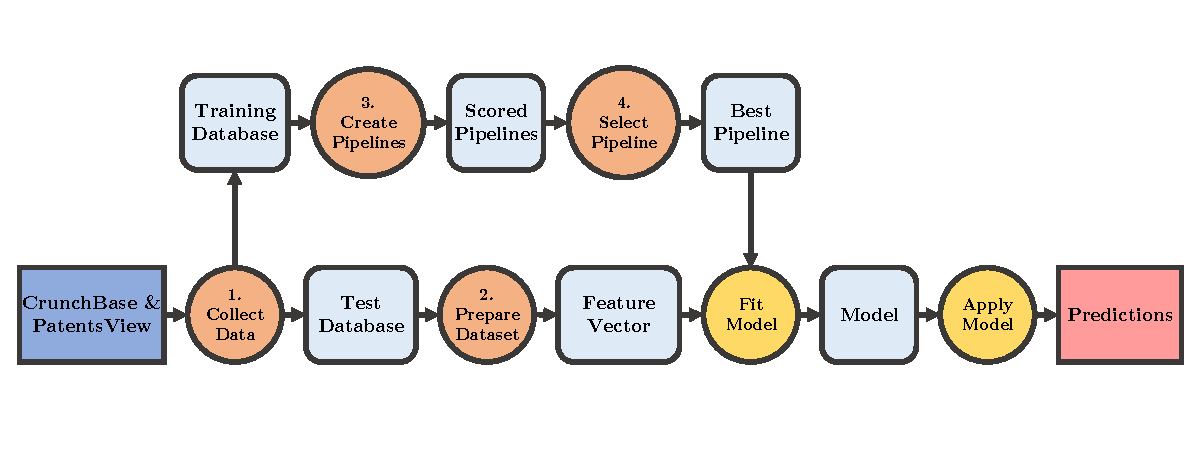
\includegraphics[width=\textwidth]{../figures/design/flowchart_make_predictions}
    \caption[Model fit and prediction flowchart]{Model fit and prediction overview. Legend: dark blue square = input, orange circle = system component, yellow circle = process, light blue rounded square = intermediate, red square = output.}
    \label{fig:design:make_predictions}
\end{figure}

\ifcsdef{mainfile}{}{\printbibliography}
\end{document}
